%
% Distributed Systems Module Book (2013-2014)
% Author: Donald Whyte (sc10dw@leeds.ac.uk)
%

\documentclass{article}

\usepackage[margin=2cm]{geometry} % easy page formatting
	\geometry{letterpaper}
\usepackage{doc} %special logo commands
\usepackage{url} % formatting URLs
\usepackage{datetime} % up-to-date, automatically generated times
% For graphic files
\usepackage{graphicx}
\usepackage{epstopdf}
\usepackage{amsmath}
\DeclareGraphicsRule{.tif}{png}{.png}{`convert #1 `dirname #1`/`basename #1 .tif`.png}

% Set the Phytitle, author, and date.
\title{Distributed Systems \\ COMP3900 -- TC31}
\author{Donald Whyte}
\date{\today}

% The document proper.
\begin{document}

% Add the title section.
\maketitle

% Add various lists on new pages.
\tableofcontents

\pagebreak
\listoffigures

% Start the paper on a new page.
\pagebreak


\section{Introduction}

A \textbf{distributed system (DS)} is a collection of independent computers that appears to its users as a single coherent system. 

It may be alternately defined as a system in which components located at networked computers communicate and coordinate their actions \textbf{only by passing messages}.

A simpler way of defining a distributed system would be one that has \textbf{no central point of failure} -- if one machine stops working, a distributed system will not be affected.

A distributed system aims to be:
\begin{itemize}
	\item \textbf{Scalable} -- as more machines are added, the system can still work \textbf{without effort} and without turning it off/modifying it explicitly
	\item \textbf{Transparent} -- you know nothing about the physical, individual systems that compose the DS
	\item \textbf{Open/Operable} -- the ability for multiple devices and services to work together to complete a common task, through the use of open standards/protocols (meaning new, different systems can communicate with, or join, the DS).
	\item \textbf{Secure} -- data and behaviour of system is protected against malicious uses without proper access. Only authorised users may access specified resources (or \textit{any} resource of the system). Paramount because machines are on a network, meaning any person/machine can communicate with the system
\end{itemize}

A distributed system must be able to \textbf{recover from independent failures} in hardware. This makes the system \textbf{robust/resilient} to failure. DSes must also deal with the inherent \textbf{complexity} that concurrency adds, whilst not having a global clock to provide a reference point for time.

Examples of distributed systems include:
\begin{itemize}
	\item The Internet (or corporate intranets)
	\item The World Wide Web
	\item A cellular mobile phone network
\end{itemize}

Note that the internet/intranets and the WWW are not \textbf{true} distributed systems, as they're \textbf{not transparent}. The URLs and IP addresses of web pages/services identify the \textbf{physical location} of the requested resource. This means you're identifying the \textbf{location of a specific independent system/component} of the whole distributed system. As such, the DS is not appearing a single, coherent system, meaning it is not a \textbf{"true"} distributed system in that sense.

The \textbf{physical architecture} of DSes tend to follow the \textbf{client-server} model, in which servers continuously listen for one-off requests from clients, providing/serving those clients with a service or resource. This is shown in Figure \ref{fig:client-server-communication}.

\begin{figure}
	\centering
	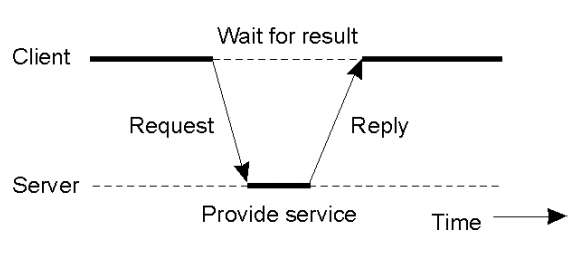
\includegraphics[scale=0.5]{figures/client-server-architecture.png}
	\caption{Client-Server Communication Architecture}
	\label{fig:client-server-communication}
\end{figure}

\subsection{The PAD Model}

Many client-server applications are constructed logically from \textbf{three} different layers of software:
\begin{itemize}
    \item \textbf{Presentation Tier} -- contains everything required to interface with the user of the system (e.g. web page)
    \item \textbf{Application Layer} -- contains the business logic layer of the application, where the \textbf{core functionality} the system provides is performed (e.g. web server script)
    \item \textbf{Data Layer} -- commits data from the application layer to a \textbf{persistent storage medium} (e.g. SQL database)
\end{itemize}

An example of a client-server system which uses the PAD model is a \textbf{web search engine}:
\begin{itemize}
    \item The \textbf{Presentation Tier} of a search engine would be the web page that the user communicates with (for example, the search page at \texttt{google.com})
    \item The \textbf{Application Tier} of a search engine would generate a query based on the users input which it would submit to the data tier. It would then take the response from the \textbf{data tier}, rank the results and provide them in \textbf{HTML format} ready to be consumed by the \textbf{Presentation Tier}.
    \item The \textbf{Data Tier} would be the database that stores web pages. It would be provided with a query from the \textbf{Application Tier}, and return a list of Web Page Titles with associated metadata (link, short description, etc).
\end{itemize}
This process, along with the logical split into the three layers is shown in Figure \ref{fig:web-search-engine-pad}.

\begin{figure}
	\centering
	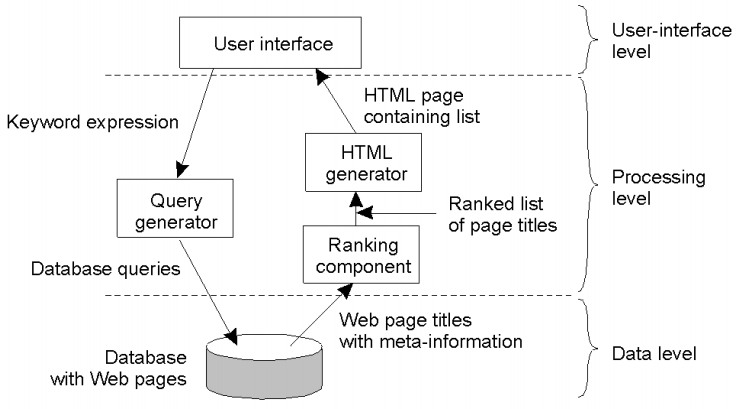
\includegraphics[scale=0.4]{figures/pad-example-web-search.png}
	\caption{Web Search Engine using PAD Architecture}
	\label{fig:web-search-engine-pad}
\end{figure}

\subsubsection{PAD and the Client Server Model}

The layers of the PAD model can be applied to the Client-Server model in \textbf{several ways}. All of the layers must be present either on the client or the server, but \textbf{how the split works} depends on the application. For example, a search engine is a typical example of where the Application and Data tiers are both provided by the server, where the Presentation Tier/User Interface is on the client machine. 

Figure \ref{fig:multi-tiered-architectures} shows the different ways in which the three layers can be split across. Notice how that some layers can be in \textbf{both} the client and the server.

\begin{figure}
	\centering
	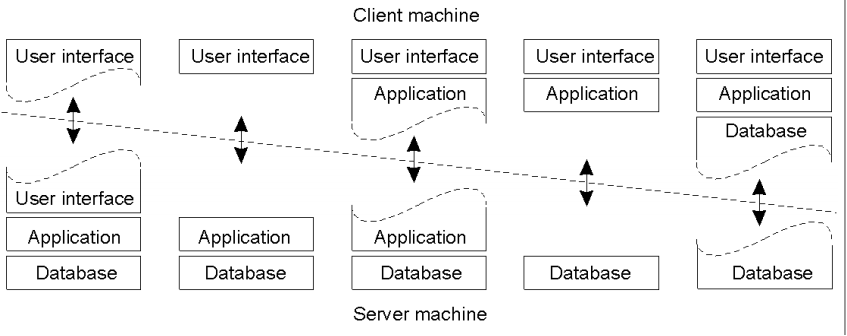
\includegraphics[scale=0.5]{figures/multitiered-architectures.png}
	\caption{Multi-tiered Architectures with the PAD Model}
	\label{fig:multi-tiered-architectures}
\end{figure}

At one extreme (left of Figure \ref{fig:multi-tiered-architectures}), the Presentation Tier may be rendered on both the Client and the Server machine (for example, when using remote desktop/VNC) with everything else being present on the server. This has the advantage of having a very lightweight client.

The other extreme (right of \ref{fig:multi-tiered-architectures}) is where a Client application has the Presentation Tier and Application Tier, and a local Database/Data Tier. This local database is sent to a Server database for backup, or for consolidation of information from multiple clients. 

Probably the \textbf{most common architecture} is to have the Presentation Tier and part of the Application tier on the client, and the other half of the Application Tier and the Data Tier on the server. Examples of this would be Web Services (for example, the Data and Application logic is partly performed by the Twitter API, but a mobile application client will also have application and presentation logic) and modern web applications (a Javascript web stack).

Figure \ref{fig:multi-tiered-client-server} shows the communicate between the three different tiers of the system (which are typically run on different machines in the system. The Presentation tier sends a request to the Application tier. The Application tier then sends a request for data to the Data Tier, which responses with the requested data. At this point, the Application tear processes the data and sends a response back to the Presentation tier, which has been waiting since its initial request.

\begin{figure}
	\centering
	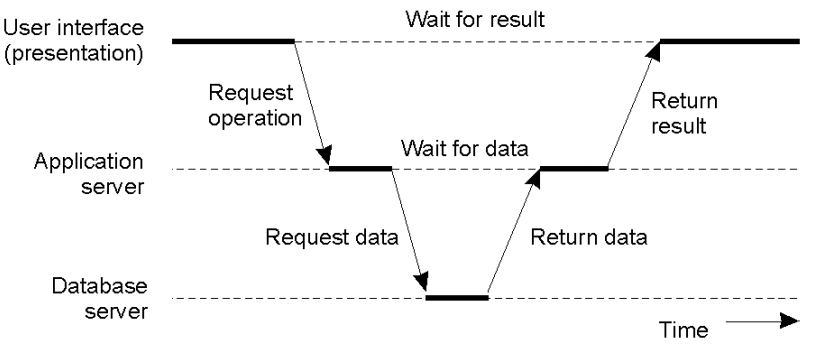
\includegraphics[scale=0.4]{figures/multitiered-client-server.png}
	\caption{A better DS: 3-Tier Client-Server Architecture 
- an example of a server acting as a client. }
	\label{fig:multi-tiered-client-server}
\end{figure} 

\subsection{Scalability}

One of the key considerations for a Distributed System is how scalable it is. A Distributed System must scale:
\begin{itemize}
    \item \textbf{In Size} --
    A distributed system can be considered to be scalable in size if it remains \textbf{effective after a significant increase} in users or resources. The Internet is an example of a system which scales exceptionally well in size. Organizing information in a \textbf{hierarchical} way improves size-based scalability (accessing it becomes $O(\log n)$ rather than $O(n)$). An example of a system which stores information in a hierarchical way is \textbf{DNS}. 

    By contrast, \textbf{single points of failure} are key problems when aiming for size-based scalability. A single server for all users, a single data repository (such as having one phone book for everyone or one instance of a database), or having to have \textbf{all information required for an algorithm on a single system/machine}. This makes it a centralized algorithm, rather than one which can perform on a subset of currently available data; this will cause scalability issues.
    \item \textbf{Geographically} -- 
    The challenge with geographically distributing a service is how to ensure that it remains \textbf{synchronized}, and managing the communication between different parts of the service. Geographically distributing 2 servers will make it much more expensive for them to communicate (longer communication times due to greater latency). This increase in network latency will also have to be taken into account for certain types of operation. For example, synchronizing data -- the original data might be \textbf{out of date} by the time it reaches another server. This is most obvious when the clocks between two machines are not synchronised, making the data out of date instantly.

    Geographic issues may also stem from \textbf{legal or political restrictions} applied in different locations, such as data storage policies (e.g. Data Protection Act 1998 in the UK).
    
    Geographically distributed services also introduce \textbf{reliability} issues.
    \item \textbf{Administratively} --
    There can be several administrative challenges as a system becomes bigger. It may have to be run in different administrative domains (e.g. countries or organisations) with conflicting policies, such as how many resources can be used, how the system is managed, and how it is secured (security mechanisms/policies).
\end{itemize}

Various strategies exist for making a system be (or appear) more scalable. For example, work could be carried out on the \textbf{Client side} rather than the server, which reduces (or delays) the communications overhead making the system appear more responsive. This also means that as there is less work per-client on the server, more clients can be added without requiring more servers/computational power to perform the work.

Alternatively, work could be completed on the Client and Server in parallel - as the user only sees the Client, they assume it is doing work (and don't have the \textbf{visible wait} whilst the server does something and the client is non-responsive).

The \textbf{distribution} of information can be organized in a hierarchical way (hierarchy of host/machines) rather than in a linear fashion in order to decrease lookup time. DNS is an example of a system which distributes information in a hierarchical way for performance (see Section \ref{sec:dns}).

\textbf{Replication} can be used so that there is not one canonical place to look up information. This allows for:
\begin{itemize}
	\item \textbf{Increased Availability} -- if the server storing that piece of data goes down, the data is still available in a replicated fashion
	\item \textbf{Load Balancing} -- allocating clients to multiple machines with the same services/data such that the balance of clients/work between the different machines is \textbf{evenly balanced}
	\item \textbf{Optimal Allocation of Servers} -- e.g. choose server geographically closest to reduce communication latency
\end{itemize}
A \textbf{local replication (cache)} is when the client machine replicates data received from the server. This can prevent the overhead of network communication completely, hiding latency issues from the client. However, replication causes a serious \textbf{consistency problems}, as all of the replicate sets must be updated when the \textbf{master} is updated (if complete consistency is required). Knowing where all the replicated data sets are can be a challenge in its own right, let alone actually sending the updated data to all the hosts such that they update it.

\subsection{Transparency}

A Distributed System should aim to be \textbf{Transparent}. A transparent system is visible to a user (or developer) as a \textbf{single platform}, rather than several discrete services which are working together. This increases the ease at which an application can be used (or developed against). There are various forms of transparency in a distributed system.
\begin{itemize}
    \item \textbf{Access} - The method in which a resource is accessed, and whether or not there's any differences in the \textbf{data representation} of that resource which should be hidden from the user.
    \item \textbf{Location} - The user should not need to know \textbf{where the resource} is located (either geographically, or in terms of servers, etc)
    \item \textbf{Migration} - An extension to Location, the user should not know if a resource has been moved elsewhere
    \item \textbf{Relocation} - It should not only be possible to migrate a resource, but migrate it whilst it's in use
    \item \textbf{Replication} - A resource should be able to be replicated across a network, without a client necessarily knowing they're accessing a replica
    \item \textbf{Concurrency} - A resource can be used by several clients in parallel, without any individual client \textbf{knowing about another client}
    \item \textbf{Failure} - The failure and recovery of a resource should not be visible to the client (good failover and fault-tolerance mechanisms)
    \item \textbf{Persistence} - The persistence mechanism (memory, disk, etc) should not be visible to the user
\end{itemize}

Many of the principles of Transparency serve as abstractions around the distributed system, so that an individual client does not need to worry about the physical implications of tasks they're completing. They can offload them to the server and only worry about the logical requirements (for example, asking the Twitter service for a tweet, rather than worrying about the individual row in a storage system like a database, that is kept in a specific server in a specific data-center in a specific geographic location). This abstraction layer also hides the underlying implementation technology of a distributed system (which may be several languages, technologies, etc). Hiding the \textbf{heterogeneity} of these systems simplifies a \textbf{client developer's job significantly}, and allows authors of the distributed system to change internal systems as required. 

When just using sockets, the FTP protocol and soon we have limited transparency, because these network services are \textbf{directly visible to the application developer}. A significant amount of explicit code is needed to establish TCP/IP communication between the client and the server. If would be nice if the use sockets could be hidden from the programmer, making it appear as if the client and server are \textbf{components of a centralised system}.

\subsubsection{Middleware}

The technologies used for providing an abstraction layer over a distributed system can be called \textbf{Middleware}. Middleware sits on top of the physical machines, to make all of them appear as a centralised system. This is shown in Figure \ref{fig:middleware}, where there are three machines which are running the same distributed applications. To the outside world, the three machines appear as a single system, but they are in fact communicating using Middleware. That is, we want hide \textbf{heterogeneity} of the underlying 
platforms from applications. Without middleware, distributed applications would be sitting directly above each individual machine, result in no transparency.

Distributed applications, which actually perform the required business logic, are built on top of the Middleware. This is done through the use of APIs, libraries and toolkits.

\begin{figure}
	\centering
	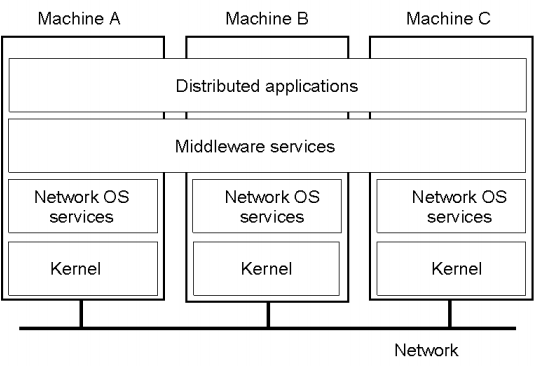
\includegraphics[scale=0.5]{figures/middleware.png}
	\caption{General Structure of a Distributed System as Middleware}
	\label{fig:middleware}
\end{figure} 

\begin{figure}
	\centering
	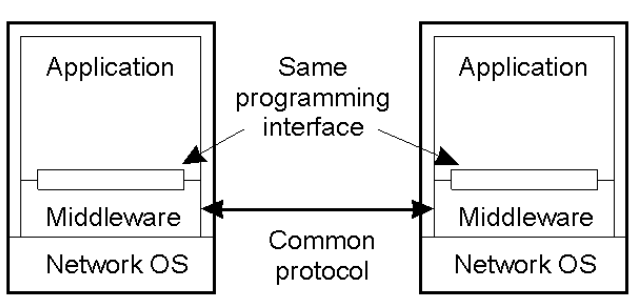
\includegraphics[scale=0.5]{figures/middleware-openness.png}
	\caption{In an open middleware-based distributed system, the 
protocols used by each middleware layer should be the 
same, as well as the interfaces they offer to applications. This makes the DS \textbf{open} for new machines to join the DS!}
	\label{fig:middleware-openness}
\end{figure} 

An example of a Middleware system is \textbf{RMI (remove method invocation)}. This allows calls to a distributed system to be abstracted into one object calling a method on another object (in much the same way as Object Orientated Programming). Invoking local and remote methods looks exactly the same -- the message is just passed over the network. This typically requires some setup code, to configure management of the remote objects themselves (their names, locations, etc.) so that methods can be invoked on them. The abstraction saves the programmer from needing to know about the \textbf{underlying network protocols}.

The object-orientated programming paradigm dominates modern software engineering. Middleware follows suit, with most middleware systems using some form of \textbf{distributed objects}. More examples of Middleware include:
\begin{itemize}
    \item \textbf{CORBA} (Common Object Request Broker Architecture) is a language and platform independent abstraction which allows multiple applications to work together towards the same goal. It is large and complex, and has fallen out of favour. It provides services for naming, persistence, transactions, etc.
    \item \textbf{Java RMI} is a method of remotely invoking methods with other Java applications. Unfortunately it is not language or platform agnostic (it's restricted to the Java VM), but it is small and simple in comparison to CORBA.
    \item \textbf{Java RMI-IIO} (Internet Inter-Orb Protocol) is a method of allowing RMI to communicate with CORBA.
    \item \textbf{DCOM} (Distributed Component Object Model) is a way of enabling remote COM calls. It works with any COM language (as its an extension of COM). It was a major competitor to CORBA, but both are now largely redundant.
    \item \textbf{.NET Remoting} is the .NET alternative to RMI. It is available to .NET languages, and is slightly more flexible than RMI.
    \item \textbf{WCF} (Windows Communication Foundation) has largely superseded other Microsoft based distributed communications technologies.
\end{itemize}

\section{Message Orientated Communication}

Interprocess communication is at the heart of all distributed systems. It describes the mechanisms/protocols used by machines to communicate with each other. \textbf{Low level message passing} on the underlying network is used to implement communication in a distributed system.

The OSI model is a seven-layer architecture which is used to implement Internet communication. The seven layers are:
\begin{itemize}
	\item \textbf{Application} -- This layer directly communicates with the user's application software.
	\item \textbf{Presentation} -– Serves as a bridge between the application and session layer, translating data from the Application layer so it's usable in the Session layer.
	\item \textbf{Session} -– Controls connections between computers, managing the connection between local and remote applications.
	\item \textbf{Transport} -– Provides transparent transfer of data between users of the system.
	\item \textbf{Network} -– Provides the means to actually transfer the data through the network.
	\item \textbf{Data Link} -– Can transfer data between network entities and detect errors in Physical layer.
	\item \textbf{Physical} -– This is the actual physical hardware the network uses: wires, wireless receivers, routers, computers and so on.
\end{itemize}

\begin{figure}[h]
	\centering
	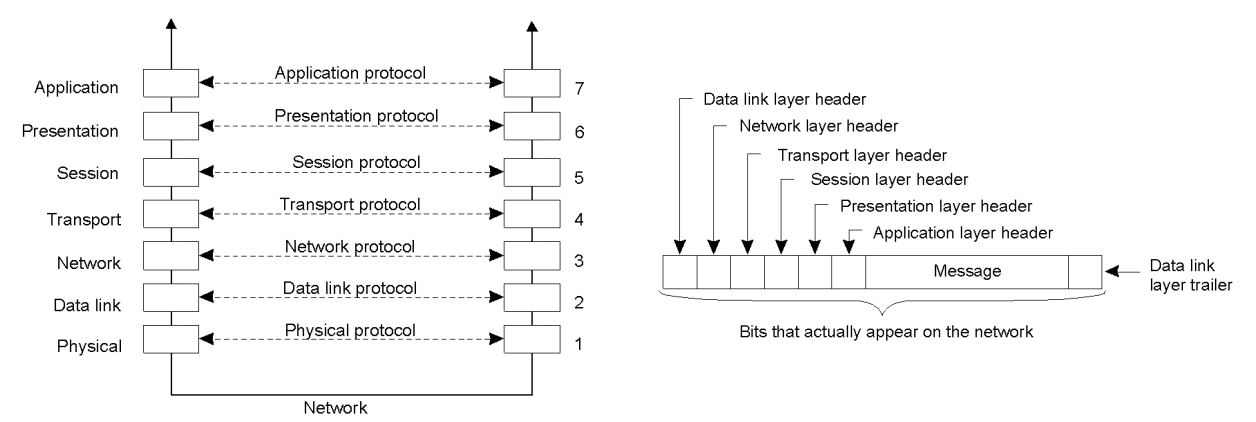
\includegraphics[scale=0.5]{figures/osi.png}
	\caption{7-Layer OSI Model for the Internet}
	\label{fig:osi}
\end{figure} 

We can \textbf{adapt} the OSI reference model to include Middleware. We replace the Presentation and Session layers with a \textbf{Middleware layer}, which sits below the Application layer and above the Transport layer (where the TCP and UDP protocols lie). This is shown in Figure \ref{fig:osi-middleware}

\begin{figure}
	\centering
	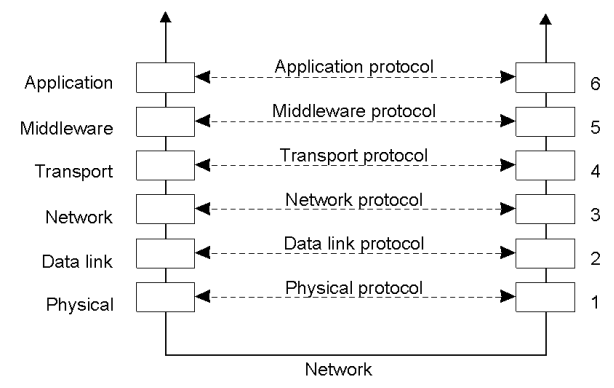
\includegraphics[scale=0.6]{figures/middleware-osi.png}
	\caption{Where Middleware Sits in the OSI Model}
	\label{fig:osi-middleware}
\end{figure} 

\subsection{Socket Programming}

Sockets are a standard introduced in 1981 to allow applications to communicate over a network or to another process. They are a relatively low-level interface which are created, used and released \textbf{explicitly by applications}. Sockets can send either TCP (reliable, byte stream orientated) or UDP (unreliable datagram) messages. 

\subsubsection{TCP}

In order to communicate via \textbf{TCP (Transmission Control Protocol)}, the client must initiate a connection with the server (via a socket designed to respond to initial requests to connect) which opens a new socket for the 2 applications (Client and Server) to communicate over. The server uses port numbers to distinguish between different clients. After the client has connected to the server via a TCP socket (and the servers IP/Port) they establish a connection and can communicate.

TCP is a stream based protocol (a stream is a sequence of characters that flow in or out of a process). There are both input streams and output streams.

To initiate a TCP connection with a server, the client and server performs \textbf{three-way handshake}:
\begin{enumerate}
	\item The client requests a connection with \texttt{SYN}
	\item The server acknowledges by responding with \texttt{SYN, ACK(SYN)}
	\item Then the client acknowledges the server's acknowledgement with \texttt{ACK(SYN)}
\end{enumerate}
After this point, a TCP connection has been established and the client and server can start sending data to and from each other.

If a client wants to close the connection, the following protocol is followed:
\begin{enumerate}
	\item Client sends \texttt{SYN,request,FIN}
	\item Server responds with \texttt{SYN,ACK(FIND),answer,FIND}
	\item Client acknowledges responses with \texttt{ACK(FIN)}, which may or may not be received by the server
\end{enumerate}

\begin{figure}[h]
	\centering
	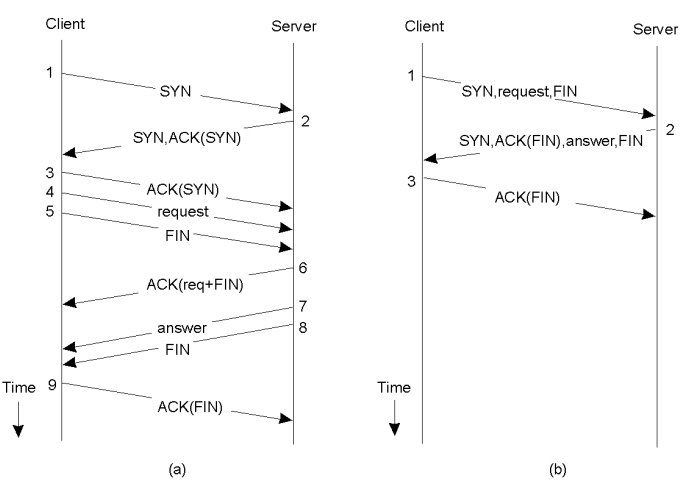
\includegraphics[scale=0.5]{figures/tcp-normal-transactional.png}
	\caption{(a) Normal Operation of TCP (b) Transactional TCP}
	\label{fig:tcp-normal-transactional}
\end{figure} 

\subsubsection{UDP}

In \textbf{UDP (User Datagram Protocol)} there is no handshaking process or `connection' between the client and server as it is an unreliable transfer of data. The client must explicitly attach the destination details (IP and port) to each packet. Because it is not a stream-orientated connection mechanism (and there is no reliability) UDP packets can be received out of order, or may be lost entirely.

\subsection{Remote Procedure Call (RPC)}

\textbf{Remote procedure calls} allow a machine to invoke a fuction/sub-routine (i.e. business logic) on another machine, passing function arguments and receiving the result back remotely. The actual function to execute is on the \textbf{remote machine}, but it is invoked on the client machine. Additionally, the results are returned on the client machine and are typically not used by the actual remote machine (unless the function has \textbf{side-effects}).

The concept of remotely calling a function can be applying to \textbf{objects} as well. You can easily have a client remotely invoking methods on an object, or remotely accessing the object's state (i.e. fields).

This is achieved through \textbf{stubs/proxies}. The client invokes a method on the proxy object (without \textit{knowing} it's going to make a remote call) and the proxy object sends off the remote method invocation message to the remote machine. This request then hits a server stub, which parses the message and calls the correct method using the correct parameters. It takes the result of the local method call and sends it back to the client in  a response. The client stub receives the response. This means that objects can be treated as local objects, even when they're actually stored on a remote component/server of the system.

\begin{figure}
	\centering
	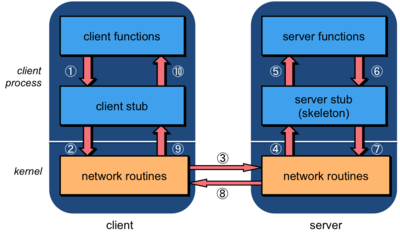
\includegraphics[scale=1.4]{figures/rpc-flow.png}
	\caption{Remote Procedure Call Components and Process}
	\label{fig:rpc-flow}
\end{figure} 

\subsection{Message-Passing Interface (MPI)}

MPI (Message Passing Interface) is a standard for passing messages between different processes. The number of processes is allocated at the start of execution, and each is given a unique ID number. The process can alternately process information, and communicate with other processes. All processes in an MPI setup run the same program (but can branch based on ID number). 

Message passing is a very portable way to create programs, as MPI is supported by various languages and platforms. It also has (fairly) simple debugging, and its easier to reason about, making it easier to create a deterministic program. 

Each process is contained within an `MPD ring'. The mpd daemon (Message Passing Daemon) runs on each machine and manages the local processes. Communication across a network with multiple hosts (all with MPD) is supported using \textit{mpdboot}.

MPI supports communication between 2 processes using a variety of commands such as \textit{MPI\_Send} and \textit{MPI\_Recv}. Both Synchronous and Asynchronous APIs are available. MPI is also capable of "Collective Communication" between all nodes, using \textit{MPI\_Bcast} and \textit{MPI\_Reduce}.

MPI is the leading standard for message passing systems, although others exist.

\section{Servlets and JSP}

Servlets are Java classes that implement a specific service via a \textbf{HTTP request}. They are subclasses of \texttt{HttpServlet} and are \textbf{mapped} to a particular URL (e.g. "/calc/add" being mapped to \texttt{NumberAddServlet} class). Each servlet class contains these methods:
\begin{itemize}
	\item \texttt{doGet()} -- Handles GET requests with mapped URL
	\item \texttt{doPost()} -- Handles POST requests with mapped URL
\end{itemize}

A \textbf{web container} are executed on web servers and \textbf{host Java web applications}. Servlet classes are compiled and installed in a web container (e.g. Tomcat), which is made accessible to clients via a web server (e.g. Apache). This is shown in Figure \ref{fig:web-container}, where there are three ways a client can \textbf{communicate with web applications} stored in a web container. A client can either directly communicate with a web container, communicate with a server who then sends a request to the web container as a client (relaying the response back to the original client) or the client can directly communicate with the server, which has a web container \textit{within} it.

\begin{figure}
	\centering
	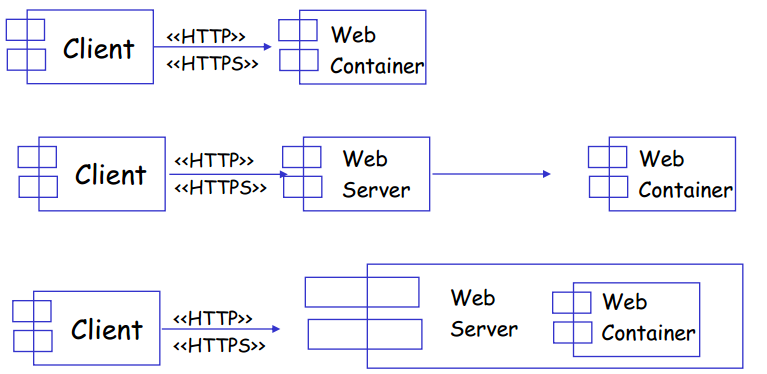
\includegraphics[scale=0.5]{figures/web-container.png}
	\caption{Three Ways a Client Can Communicate with a Web Container}
	\label{fig:web-container}
\end{figure} 

One way of \textbf{installing} servlets into a web container is to package a collection of servlets as a \textbf{web application} in a Java \textbf{WAR (Web Archive}) file. This is similar to a JAR file, but used specifically for Java web applications by web containers.
\textbf{JSP} stands for Java Server pages and is way of embedding business logic into the presentation layer (i.e. web pages) of the web application. You embed Java code into special HTML tags, which gets executed when the web page is requested. The output of the executed code is placed in the spot where the Java code was in the document. Figure \ref{fig:jsp-processes} shows what happens when a user requests a service that is represented as JSP file. It is processing using a \textbf{JSP Translator}, which takes a JSP file, executes the Java code inside it and replaces said Java code with code's output.

\begin{figure}
	\centering
	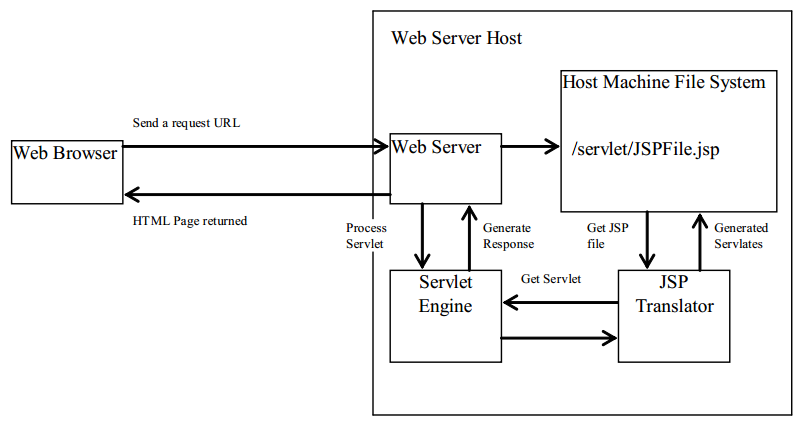
\includegraphics[scale=0.5]{figures/jsp-processing.png}
	\caption{Process of producing a HTML response using a JSP file (e.g. request to URL \texttt{http://www.server.com:8080/servlet/JSPFile}}
	\label{fig:jsp-processes}
\end{figure} 

Using servlets and JSP allow you to write pages of HTML with \textbf{embedded servlet API calls and raw Java logic}. However, this has the following \textbf{disadvantages}:
\begin{itemize}
	\item Servlets are tedious to write when the presentational code \textbf{dominates} the application (have to manually write Java code that implements complex HTML/JavaScript tags)
	\item It is desirable to have a \textbf{cleaner separation of logic from markup}, allowing the interface to be developed:
	\begin{itemize}
		\item without the need to \textbf{recompile source code}
		\item without need for \textbf{high expertise in Java programming} (so web designers can work on the front-end web pages without worrying about complex, technical business/application logic)
	\end{itemize}
\end{itemize}

\section{RMI}

RMI (Remote Method Invocation) is a way of abstracting network communication into calling a method on an object. An object will typically reside on one server, and interfaces to that object will be made available across the distributed system. A remote object is used to describe an object on a remote server, which is accessed via the interfaces that are sent across to all clients. 

A \textbf{interface} to an object specifies what an object's methods do and how they are called. An interface \textbf{does not} specify how methods must be implemented, or how an object must represent its state (fields). A give object may be accessible via multiple interfaces, and more than one kind of object may realise a given interface (many-to-many relation between interfaces and classes). Because the iterface and implementation are separate, they can \textbf{reside on different machines}. This means you can have the interface for an object on the client and server, but just have the server contain the implementation class (the client doesn't need to know \textit{how} it is implemented, just that the required behaviour/logic is there to be called).

An object's interface must be \textbf{described to clients}. This is done via an \textbf{IDL (Interface Definition Language)}. An IDL is particularly useful when a distributed system constitutes of multiple languages, technologies or platforms. The implementation of the object can be written in any language/platform which supports the chosen IDL. This is particularly useful when ineracting with legacy systems that you use very old technologies that don't match the technology your new systems use.

\subsection{Transience and Persistence}

A \textbf{transient} object is destroyed when the server managing it is terminated. A \textbf{persistent} object survives past the lifetime of its current server. A persistent object has to be stored somewhere (usually a database), so that a new server can pick it up later. 

\subsection{Serialization (Data Marshalling)}

Objects must be \textbf{marshalled/serialized} so that they can be passed across a network. This is the process of converting Java objects into a stream of bytes; this serial data structure is easy to send across the network.

Serialization typically takes a \textbf{"deep copy"} of an object, which makes it a very expensive operation, since an object may contain references to other objects, which can lead to the entire object graph of the application being serialized.

Fro (RFC 2713):
\begin{quote}
To \textbf{"marshal"} an object means to record its state and codebase(s) in such a way that when the marshalled object is "unmarshalled", a copy of the original object is obtained, possibly by automatically loading the class definitions of the object. You can marshal any object that is serializable or remote. Marshalling is like serialization, except marshalling also records codebases. Marshalling is different from serialization in that marshalling treats remote objects specially. 

To \textbf{"serialize"} an object means to convert its state into a byte stream in such a way that the byte stream can be converted back into a copy of the object.
\end{quote}

In other words, the \textbf{difference} between marshalling and serialisation is that marshalling transforms the object's class definition/implementation (i.e.  \texttt{.class} file) \textit{as well as} the object's state into a stream of bytes. The remote server can then \textbf{automatically load} the serialised class and then use that class to reconstruct the serialised object instance. Serialisation itself only converts the \textbf{state of a specific object} to a stream of bytes. It does not sent the class definition.

\subsubsection{Bytestream}

An object can be serialized into a stream of bytes and transmitted across to other machines. This is generally very efficient in terms of network overhead, as the object is sent in a very compressed form. It is also much less expensive to serialize and deserialise the object, as parsing is simple. However, bytestreams do not tend to be a very \textbf{portable} method of transferring objects, as the byte representation of objects will be different depending on the languages or platforms involved (.NET, Java and C++ all store objects in very different ways). Different platforms may also store primitive data types in different ways. For example, different processor architectures may store integers using big or little endian, or store floating point numbers differently. The client and the server must agree on the message format beforehand.

Java allows an object to be serialized if it implements the \textit{Serializable} interface. The bulk of the work is carried out by the \textit{ObjectInputStream} and \textit{ObjectOutputStream} classes (with Output Streams serializing, and Input Streams deserializing). The \textit{writeObject} and \textit{readObject} methods on those objects are used to serialize and deserialize specific objects. 

Certain properties may not need to be serialized. These can be marked as \textbf{transient} (using an Attribute/Decorator). 

\subsubsection{XML}

XML (Extensible Markup Language) is a text-based serialization format. It is a form of extensible markup which is designed to be readable by both machines and humans. Most programming languages support XML, having comprehensive support for serializing and deserializing into the format, making it a reasonably good choice for cross-platform development (although some criticism comes from the slow parsing speed, which is necessary in comparison to Bytestreams), and it has standardized ways of representing integers, floating points and other data types.

\textbf{Extensibility} is one of the key attributes of XML. It can be used to express various documents and data structures, providing they have a hierarchical structure (as XML is inherently a tree). This allows it to express object graphs reasonably well (although some XML parsers can struggle with cyclic references). Custom schemas can be created for XML (through Document Type Definitions, or DTDs, or XML schemas, or XSDs), which can be enforced by parsers. This allows systems to publish the schema of XML that they support, and \textbf{require that clients follow that schema}.

Whilst XML does have a method of serializing integers and floating point numbers (amongst other types), it has no actual support for them inherently. This can lead to parsers not knowing what to deserialise a type to (is it an int, or a numerical string?). XML is also sometimes criticized for being needlessly verbose, which can decrease the human readability and increase the required bandwidth to send messages.

\subsubsection{JSON}

JSON (JavaScript Object Notation) is an alternative text-based data serialization format, which is inspired from the object literal syntax is JavaScript. As such, it has defined data-types (string, number, date, array, object (or dictionary) and null) which vastly decreases the likelihood of data being incorrectly parsed. The simplicity that this affords is often cited as making parsing faster and easier (as basically all languages have native support for JSONs data types in some form or another), with some languages supporting JSON natively (such as JavaScript and Python). This advantage is most notable next to XML, where parsers have to define custom types to represent XML specific concepts (such as Documents, Nodes, CDataSections, etc).

JSON is also generally less verbose, being a more lightweight solution, which can aid human readability and makes it use less bandwidth. Web development, particularly the proliferation of web services and communicating with them using JavaScript and AJAX has seen JSON become one of the main serialization forms used.

However, the cost of JSON being more lightweight is a \textbf{lack of formality}. It has no support for the extensible features of XML, such as the ability to define custom schemas for validation. It also provides no functionality for attributes - it is a simple key-value pair mechanism of storing data (although values can be complex data types, such as arrays or nested objects).

\subsection{Java RMI}

Java has a specific implementation of RMI. As a `Java-only' solution, it is much simpler than a language independent solution such as CORBA. It is designed to fit in with the Java language as seamlessly as possible -- calling a method on a remote object \textbf{appears identical} to calling a method on a local object (as remote and local objects are type-equivalent). 

\subsubsection{Remote Object References}

In order to call methods on a remote object, the client must have a unique reference to the object. These references are called \textbf{Remote Object References (ROR)}. This is a \textbf{transparent} mechanism of accessing or referencing an object, as ROR is the only way of referencing objects.

In order to ensure stability and correctness, each ROR must be completely unique. Even after an object is disposed of, its ROR should never be used again because an obsolete reference may exist elsewhere in the system. 

Various methods could be used to generate an ROR. A GUID/UUID could be generated for each object. Java \textbf{concatenates various attributes} about the current system to generate the ROR, which are:
\begin{itemize}
	\item Internet address of machine hosting the object (32 bits)
	\item Port number associated with server managing the object (32 bits)
	\item System time (32 bits)
	\item Object numbers (32 bits) -- causes \textbf{numerical overflow} if DS runs for too long
\end{itemize}

This would appear to be a fairly reliable way of generating a unique identifier as the IP identifies the machine, the Port identifies the application and the System Time and object number provide uniqueness local to that process on that machine at that given time. Feasibly, \textbf{collisions could exist} if the IP address is reassigned to another machine with a different system time, or if the time of the original machine is changed. 

Rather than have the overhead of looking up a Remote Object Reference, local objects are typically copied \textbf{"by value"}. The actual object itself is sent as a parameter (as in a typical method call), rather than the remote version of it. This is you don't need to perform a \textbf{remote call (i.e. network request} \textit{every} time you invoke a method on an object. Copying the remote object to local memory may initially take more time, but could save time through reduced overheads in the future.

Because of the cost of serialization, it is more expensive to send an object than a primitive value. In contrast, when sending a return value it is much less expensive to send an object than a series of primitive values. Whilst the object will still take up more bandwidth, each return value requires an individual remote method call, and the overhead of this is greater than the extra bandwidth used.

\subsubsection{Proxies, Stubs and Skeletons}

\begin{figure}[h]
	\centering
	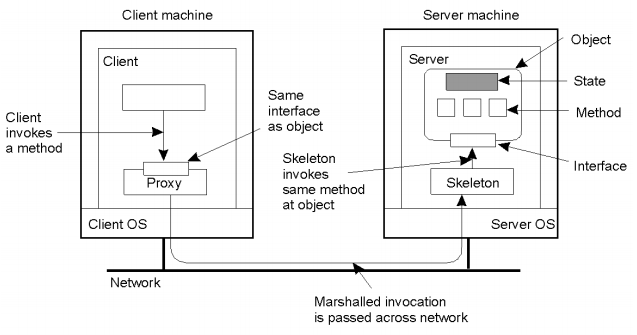
\includegraphics[scale=0.7]{figures/rmi-architecture.png}
	\caption{RMI Architecture}
	\label{fig:java-rmi-architecture}
\end{figure} 

Figure \ref{fig:java-rmi-architecture} shows the architecture of Java RMI. The client accesses a proxy object that implements the same interface as the real object. It calls methods on the proxy object, which delegates the task to the remote object using message passing. The server then receives this message and determines which object and method of chosen object to call, return the result back to the client via another message. More specifically:

A ROR is not seen directly, as this would not be very "friendly" to program against. Instead, the ROR is used to create a \textbf{Proxy} or \textbf{Stub} object, which has access to the ROR and can therefore \textbf{route calls} to the appropriate remote object. The proxy object has the same interface as the remote object (making it transparent in code through polymorphism). When a method is called on the proxy, it will \textbf{marshal} (serialise) the client method invocation into a series of messages (typically streams of bytes) and send them to the remote object. When it receives a response it will \textbf{unmarshal} (deserialise) the response. This has a lot in common with the "traditional" view of Object Orientation as message passing.

When the server receives the message, a \textbf{skeleton} object unmarshals the message and does the actual method invocation requested (calling the real object on the server). The return value is then marshalled by the skeleton, and sent to the clients proxy object. This sequence of events is also shown in Figure \ref{fig:rmi-event-sequence}. 

\begin{figure}
	\centering
	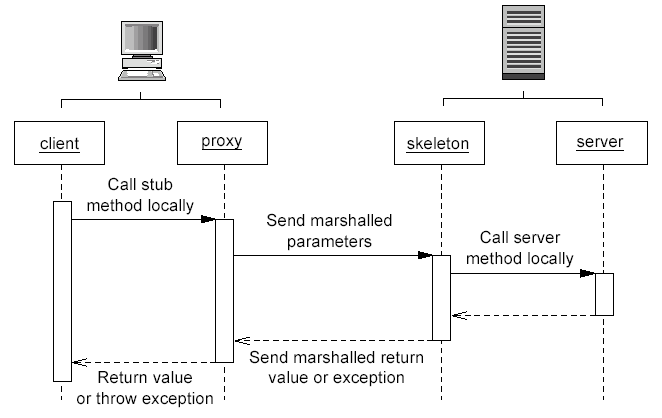
\includegraphics[scale=0.5]{figures/rmi-event-sequence.png}
	\caption{Sequence of Events when a Remote Method is Invoked in Java RMI}
	\label{fig:rmi-event-sequence}
\end{figure} 

\subsubsection{Classes and Interfaces}

There are various classes and interfaces in the Java implementation of RMI.

A user specified interface is used to \textbf{describe the methods and properties} of the remote object. This interface must inherit from the \texttt{java.rmi.Remote} interface. Methods must potentially throw the \texttt{java.rmi.RemoteException} to indicate that something has gone wrong with the remote invocation of the method. A client must be prepared to handle the \texttt{RemoteException} as well as any application-specific exceptions. There may be little or no information on whether the call succeeded or failed when a \texttt{RemoteException} is thrown, so the client and server must be designed with this in mind. 

The actual class implementation of the remote object should inherit from \texttt{UnicastRemoteObject}. This makes the object \textbf{accessible remotely} on a host-to-host basis. An object instance must be alive when the service is requested, and must be reachable using TCP/IP. If the object can be persisted (e.g. stored in a file or database), it should inherit \texttt{Activatable}.. Having your RMI class extend \texttt{MulticastRemoteObject} allows the object to be replicated across multiple machines (for greater fault tolerance).

\begin{figure}[h]
	\centering
	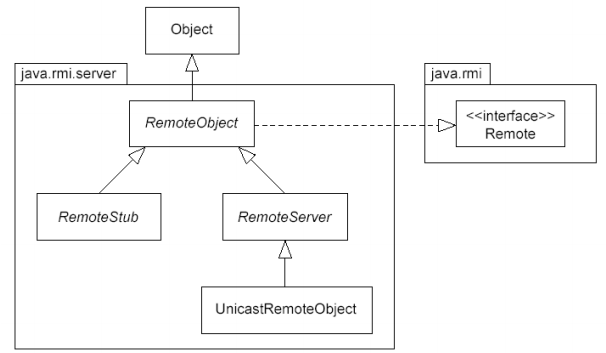
\includegraphics[scale=0.5]{figures/rmi-java-classes.png}
	\caption{Java RMI Classes}
	\label{fig:rmi-java-classes}
\end{figure} 

Previously, a separate compilation step would be used to generate the Proxy/Stub code, but it is now generated as part of the standard Java compilation process. 

\subsubsection{Registry Service}

A \textbf{registry service} is used to locate other objects (using their Remote Object References). A server in the DS \textbf{registers} objects within the registry, giving each a unique name. The client \textbf{looks them up by names}. Note that these names are not the RORs that RMI  maintains internally (as clients do not know about those names).

The registry is \textbf{not a general naming service} -- it is designed to hold a \textbf{few objects} which reference the other objects in the distributed system. This solves the problem of trying to find the first item in the distributed system (without having its RoR) so that other objects can be found. The registry should not contain all of the objects in the system. Another way of thinking about it is that the RMI registry is intended to support \textbf{hierarchical object structures}, with the root objects being registered in the registry and the child objects accessible via the root objects.

As the registry is not a general object-finding service, it will typically return a \textbf{factory object} which can be used to bootstrap the rest of the distributed system.

\paragraph{\textbf{NOTE: }} The \texttt{rmiregistry} must be started before the server. 

There are various \textbf{security issues} with the registry. Any program that runs on the same host as the registry can bind, unbind or rebind any object. Any client can look up objects in the registry. This could cause application-critical objects to be rebound with malicious objects by a compromised application on the same host, or an application getting a reference to an object and manipulating the distributed system's state.

This means a client could be remotely executing a method of an object, thinking it's going to do a particular task when in fact is does something completely different due to code injection. An example of this is an \textbf{authentication} object for a bank in which the client sends their username and password. The remote object may have actually been replaced by a malicious user, where the new object simply \textit{saves} the user's details for later use.

A \textbf{security manager} can be installed on the clients, which stops network connections to particular hosts (e.g. if remote object is not on particular servers) unless they're \textbf{explicitly enabled in a policy file}. The security manager is only required on the registry if it also has a client installed on the same host. It is also not required if a client has all of its required objects locally (including any stubs). 

\subsection{Designing for RMI}

There are often cases where an application consists of operating on a set of elements. For example, a simplified model of banking can be seen as operating on a set of \textbf{Bank Accounts}. There are two primary ways to design a Java based RMI system to deal with a set of objects.

\begin{itemize}
    \item \textbf{Multiple Individual Objects} -- in the example above, this would be having a remote object for every bank account
    \item \textbf{One Collection Object} -- this would be having a single remote object representing the set of objects. In the above example, this would be having a Bank remote object, which gives access to accounts. An alternative would be to have a subset of objects (i.e. multiple "bank" objects each responsible for a subset of all accounts in the system).
\end{itemize}

The two architectures differ in several ways. Depending on the application, different architectures will be more or less suitable. 

\begin{itemize}
    \item \textbf{Scalability}
    Individual Bank Accounts are self-contained, location independent objects. They can therefore be distributed across physical machines relatively simply -- the objects just need a JVM on any physical machine, and they can be registered in the distributed system. By contrast, a bank object is a \textbf{monolithic object} which does not spread to multiple servers very well. If a bank is spread across two servers, clients could access both simultaneously and try and access the same account, causing \textbf{consistency problems} (such as the account going overdrawn). This need to enforce consistency makes a bank object inherently less scalable. 

    \item \textbf{Multi-Account Transactions}
    Some transactions will inevitably involve multiple accounts. Depending on the type of transaction, accounts will need to either be accessed in serial (e.g. removing 100 from account A, depositing 100 to account B) or will involve simultaneous access to several accounts (transfer from account A to account B). If the accounts have to be accessed in serial, then there will \textbf{not} be a significant performance difference regardless of the architecture (except for the cost of acquiring references, which only has to be done once for a bank). If accounts are accessed simultaneously there may be a significant performance difference. In the case of an inter-account transfer, \textbf{two remote calls} would be needed if every account has its own remote object, where with a bank it could be completed in one request (single \texttt{transfer()} remote call). This difference would be more pronounced where lots of accounts are involved (for example, a payroll). 

    Some consideration should be given to the fact that transfers between accounts are probably less common than simple deposits and withdrawals.

    \item \textbf{Reliability}
    If all of the Account objects are stored within one server (the bank) then there is a \textbf{single point of failure} in the system. It is sensitive to hardware (or JVM) failure, and risks corrupting a lot of data. The inherent complexity associated with having a Bank object may also increase the likelihood of failure. On the other hand, if each Account has its own server then an issue with one account is isolated to that account, limiting the damage that any failure can cause. In essence, Accounts are sand boxed from each other due to the distributed nature of the objects.

    Another issue may arise in the case of joint bank accounts (or other places where an account could be accessed twice at the same time). If 2 people access an account, they are assigned different threads. These threads may interrupt each other or generally act in a way which corrupts the state of the account (essentially standard concurrency problems - deadlocks, race conditions, etc).
\end{itemize}

\textbf{Indirection} is when you send off multiple requests/tasks \textbf{in bulk}, as a single request to a \textbf{proxy}, who then sends all the individual requests to the desired machines (see Figure \ref{fig:indirection}). The reason you may want to do this is to minimise the number of requests over a \textbf{WAN (wide area network)} by having the proxy be physically close to the target machines. That is, the proxy is connected to the target machines over a \textbf{LAN (local area network}). This reduces the network communication overhead that can occur when performing large amounts of requests.

\begin{figure}
	\centering
	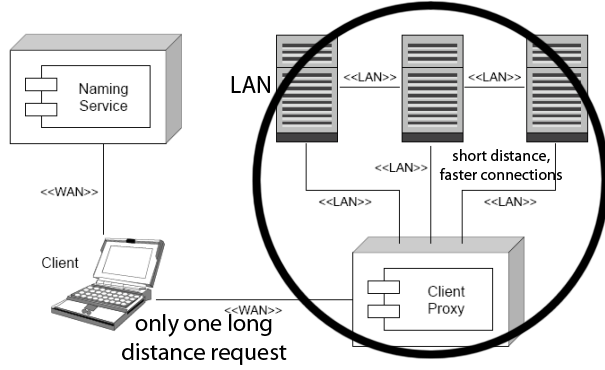
\includegraphics[scale=0.5]{figures/indirection.png}
	\caption{Indirection as Technique to Reduce Number of Requests over WAN}
	\label{fig:indirection}
\end{figure} 

\subsubsection{Performance Questions}

Be sure to always \textbf{relinquish} your remote references by setting the remote object to \texttt{null} when you know you're done with them. This means that the remote object will be cleaned up/destroyed as the garbage collector knows that it is not needed any more.

With RMI, passing two primitive value arguments is often \textbf{cheaper} than passing one combined argument (object). With \textbf{returned values} however, it is the opposite. Returning two distinct values requires two remote method calls (as each call can only return one value), which can be very expensive. It is common to create a class that contains all of the return values in it and then send that object off as a return value.

\section{Service Orientated Architecture}

A software system can be thought of as a series of components which cooperate to achieve a goal (or to "service the needs of the system environment"). Conceptually, software systems can be decomposed into three layers. The Presentation layer, Application layer and Resource Management (data) layer. These layers logically separate the functionality of a software system. When implemented, the layers can be combined in different ways, referred to as \textbf{"tiers"}.

There are primarily 4 different basic types, based on the number of tiers. 

\subsection{1 Tier}

\begin{figure}[h]
	\centering
	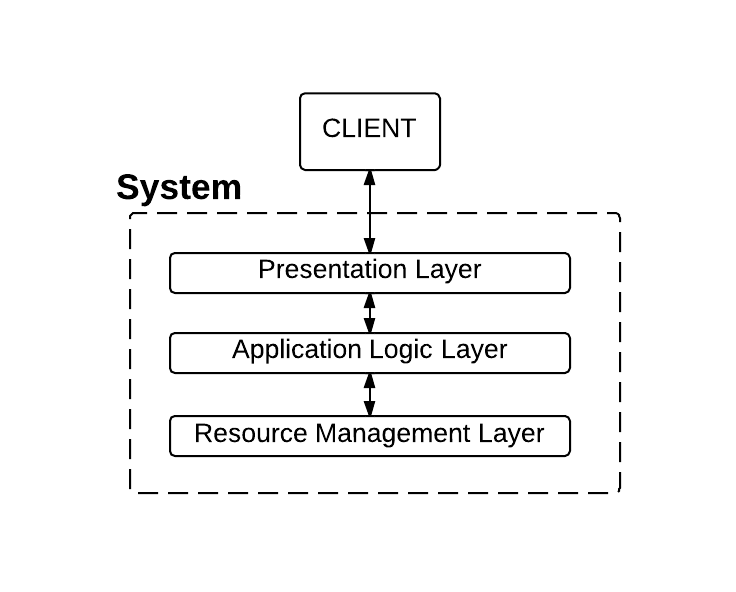
\includegraphics[scale=0.3]{figures/1-tier.png}
	\caption{1-Tier Service Orientated Architecture}
	\label{fig:one-tier-architecture}
\end{figure} 

1 Tier software systems are typically legacy applications created on mainframes. An unintelligent client will connect to the mainframe which allows the user to communicate with the system (e.g. via command line), but fundamentally everything takes place on the mainframe. The single tier (the mainframe) contains the logic for all 3 layers. 

This is a fundamentally monolithic approach to software design, which places an emphasis on efficient use of software resources, and places all of the \textbf{cost} in one machine (the mainframe, which acts effectively as a "server") rather than having to have similarly expensive/powerful clients (as there is almost always more clients). However, the monolithic nature of 1 Tier systems makes them difficult (and expensive) to maintain.

\subsection{2 Tier}

\begin{figure}[h]
	\centering
	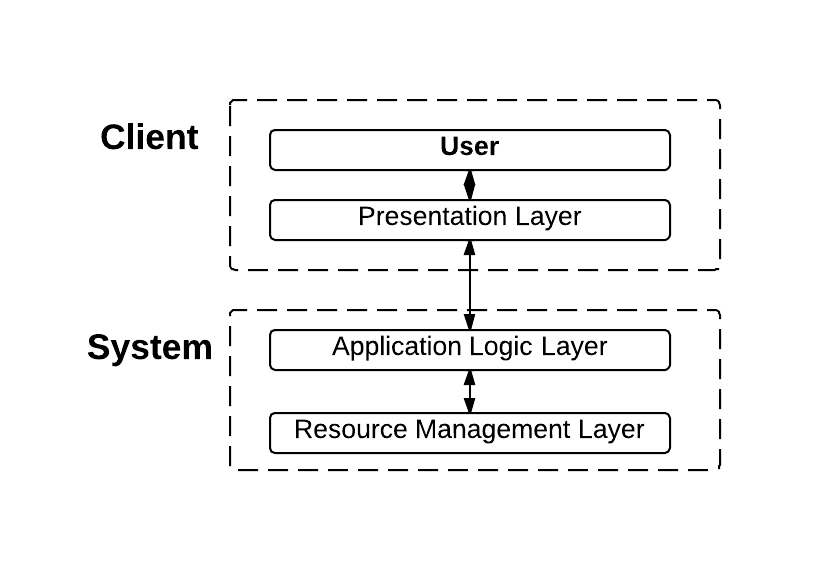
\includegraphics[scale=0.3]{figures/2-tier.png}
	\caption{2-Tier Service Orientated Architecture}
	\label{fig:two-tier-architecture}
\end{figure} 

With the advent of the PC, unintelligent terminals declined in popularity and the presentation layer was moved away from the centralised mainframe, and towards the (now more powerful) \textbf{client machines}. This allowed the presentation layer to utilize the newly available power of the client, but also allowed for a more flexible presentation tier, as it could be modified without increasing the complexity of the rest of the system. Different clients could have completely different presentation tiers, but use the same underlying system. This has become a popular architecture, particularly within client-server architectures. 

As the number of clients increases, the performance overhead of the server can become problematic. Applications on the client side may also outgrow the server side portion of the application, meaning the client-side \textbf{requires functionality which does not exist in the other tier of the system}. This can lead to the presentation layer in the client calling multiple servers, each with different application logic. This approach causes heavier client applications, which are complex and \textbf{dependent on several different services}.

Furthermore, the client has to carry out tasks which would typically be part of the application logic in order to \textbf{tie} together different services, and the \textbf{network load} between the client and server may increase.

Custom code added to clients to glue together services is also not reusable. As the client uses more and more services, it grows in complexity until it becomes difficult to maintain.

\subsection{3 Tier}

\begin{figure}[h]
	\centering
	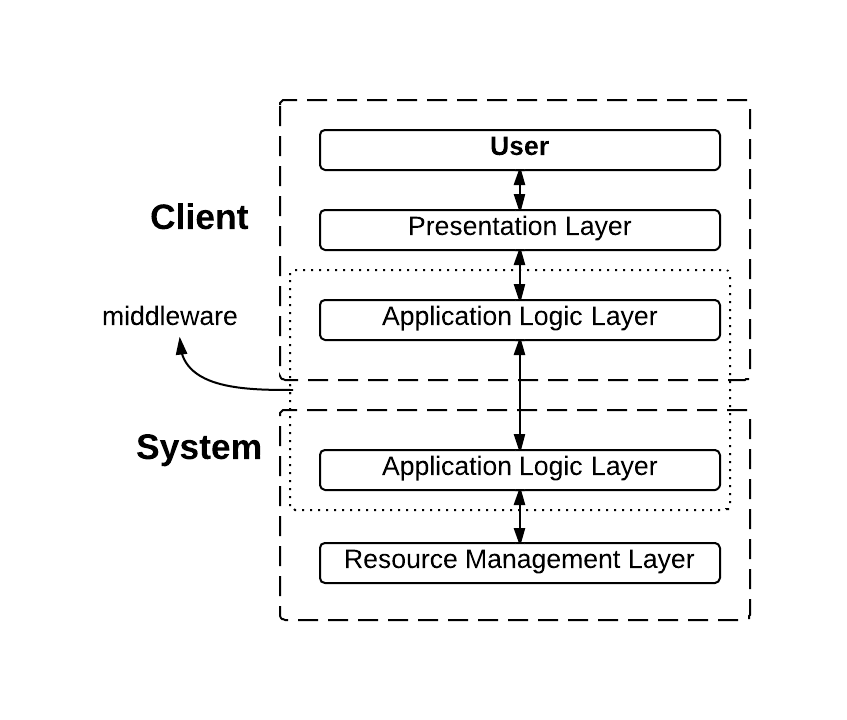
\includegraphics[scale=0.3]{figures/3-tier.png}
	\caption{3-Tier Service Orientated Architecture}
	\label{fig:three-tier-architecture}
\end{figure} 

In order to overcome the problems of 1 and 2 tier systems, 3-tiers systems were developed. The \textbf{3 Tier architecture} provides a clean separation between each of the layers, giving the application logic its own tier which sits in-between the client and any back-end resources required.

This "middleware" allows the presentation tier on the client, and the data tier on a server to adapt and change \textbf{independently} of each other. It forces the presentation tier to access the application/middleware tier, rather than the data tier directly, reducing the likelihood of \textbf{"fat" clients}, the number of dependencies that the presentation tier has, and the lack of re-usability associated with putting application logic directly in the client. 

3 Tier architectures are primarily intended to \textbf{integrate} different things together. The application tier can access several different data sources, and be accessed by several different clients. This decoupling is a powerful abstraction which simplifies software design.

However, it can be difficult to integrate some systems together. Sometimes, \textbf{existing 3 Tier systems} must be integrated \textbf{together}, or integration must take place with systems available over the Internet (rather than in a trusted, controlled networking environment). This problem is exacerbated by a \textbf{lack of standards}. There are a variety of interfaces and communication protocols which could be used to integrate systems.

\subsection{N Tier}

\begin{figure}[h]
	\centering
	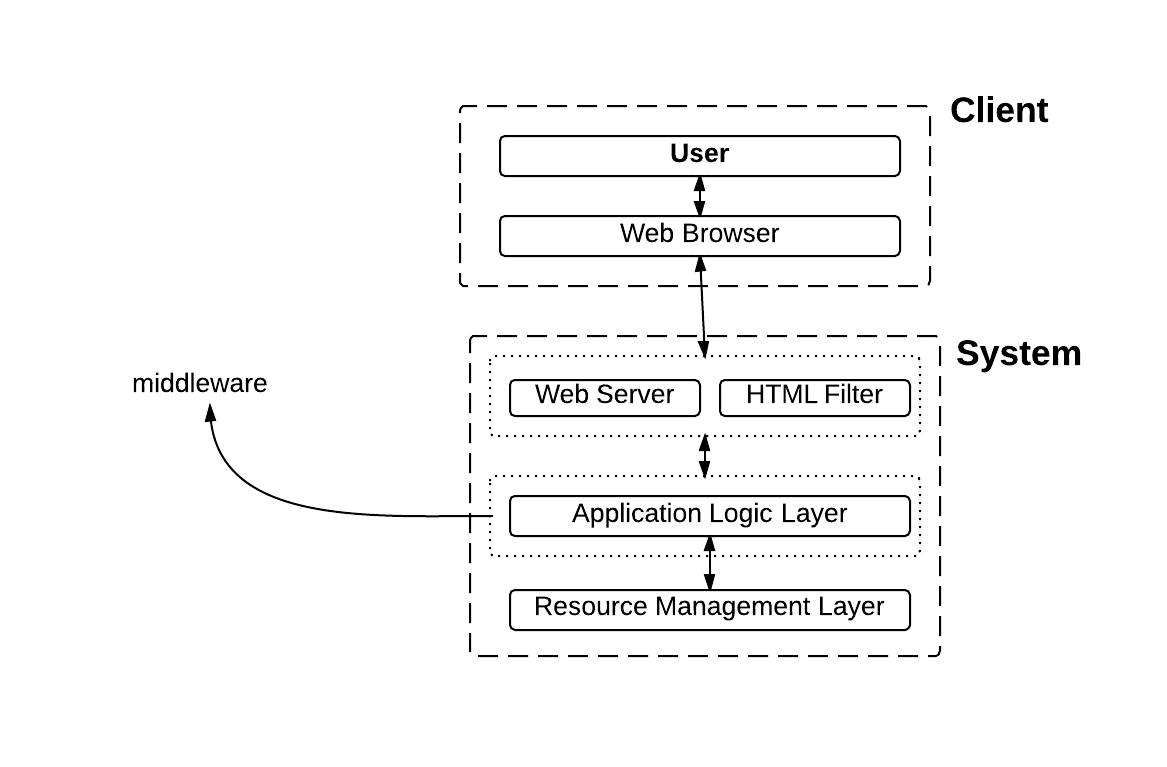
\includegraphics[scale=0.3]{figures/n-tier.png}
	\caption{N-Tier Service Orientated Architecture}
	\label{fig:n-tier-architecture}
\end{figure} 

N Tier architectures aim to \textbf{generalize} even further, to allow for integration between multiple 3 Tier systems. The requirement for an N Tier architecture may stem from either:
\begin{itemize}
    \item The need for an application to communicate with a 	\textbf{more complex data source}. Rather than just communicating with a database, an application may need to communicate with an existing 2 or 3 Tier system to access resources. For example, many modern web services (such as Twitter) are complex 3 Tier (or N Tier) systems themselves, but are used by other applications as a data layer.

    \item An \textbf{additional tier} may be added by incorporating a web server into the presentation layer. As web servers are so complex, they can be regarded as a separate tier entirely. An example of a web server that may grow in complexity is \textbf{Apache} -- the logic and settings behind a particular configuration may be so complex (complex URL mapping logic), it could be considered another tier itself.
\end{itemize}

Whilst N Tier architectures have evolved as a response to the issues with 3 Tiered systems, they still face some of the same issues. The \textbf{lack of standards to facilitate interoperability} will still cause problems in the disparate systems of an N Tiered application. Additionally, it highlights the \textbf{large amount of middleware} required to get multiple systems working together in a coherent fashion. This is especially true when there are multiple machines involved, each of which may be using custom middleware (requiring middleware between the middleware layers).

\subsection{General Trends}

It is clear that over time software systems have evolved from monolithic solutions implemented on one machine (usually a mainframe) to complex and decoupled systems with many tiers. Over time, software systems are increasing in complexity, but still need to be integrated with existing (sometimes legacy) applications. The Internet has enabled applications to connect together, changing the emphasis of software development from making individual, standalone systems to a collection of integrated applications, running in different physical, administrative and organizational locations. 

There are still issues remaining. Chief amongst them is the \textbf{lack of standards} when communicating between systems. There is also the challenge of integrating different systems from different administrative domains. 

\subsection{Services}

As a way of responding to the issues of conventional, tiered systems, many applications are now being developed using \textbf{service orientated architectures}. Service orientated development encourages applications composed of \textbf{several dynamic, loosely coupled services}. These services may exist in any organization. Services are invoked through \textbf{messages}, rather than the traditional object-orientated approaches.

A \textbf{service} is defined via a contract. If the correct requests are sent, responses will be returned from the service \textbf{as expected}. That is, a service publishes its required inputs and expected outputs and is stating that it will \textbf{follow that specification} when a client invokes the service.

\begin{figure}
	\centering
	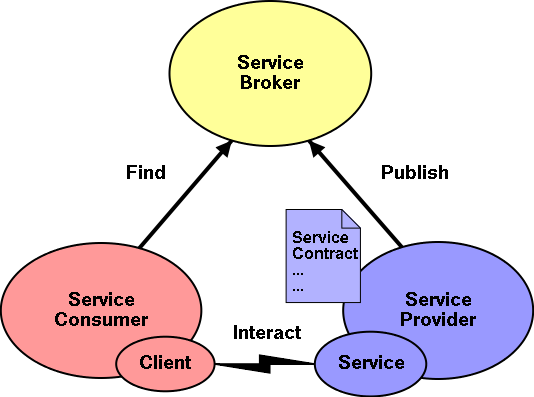
\includegraphics[scale=0.4]{figures/soa.png}
	\caption{Typical Service Orientated Architecture}
	\label{fig:soa}
\end{figure} 

Figure \ref{fig:soa} shows the service orientated architecture. There are 3 roles for participants in a Service Orientated Architecture:
\begin{itemize}
    \item The \textbf{Provider} publishes the service (via a Broker)
    \item A \textbf{Broker} acts as a \textbf{directory} for services
    \item The \textbf{Requestor} uses a broker to find, bind to, and use a service.
\end{itemize}

A service consumer (requestor) understands the contract the service implements, and adheres to the policy specified in the contact. The requester also \textbf{binds} to the service's \textbf{endpoint}, which is virtual identifier specifying the \textbf{location} of the resource. This is shown in Figure \ref{fig:soa-provision-and-consumption}.

\begin{figure}
	\centering
	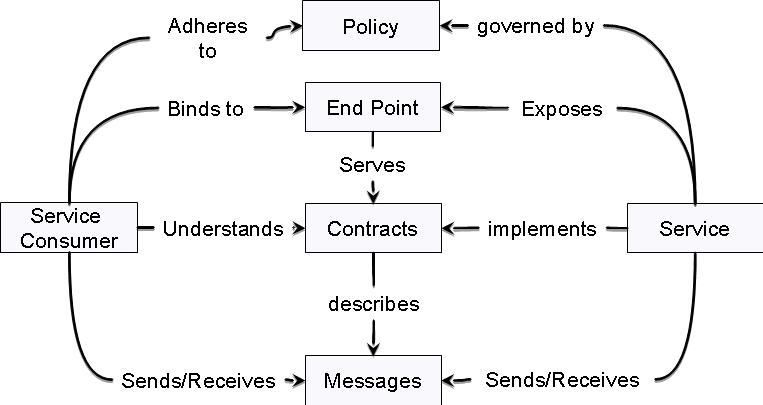
\includegraphics[scale=0.4]{figures/soa-process.png}
	\caption{Provision and Consumption of a Service using a SOA}
	\label{fig:soa-provision-and-consumption}
\end{figure} 

The primary differences between Services and traditional Tiered architectures are as follows:
\begin{itemize}
    \item \textbf{Decentralized Middleware} -- In a tiered system, there is no obvious place to put a piece of middleware to support communication between 2 different organizations. Services expose an endpoint which any client can bind to, and the necessary functionality for finding other services and communicating with them is present in \textbf{each service}. This allows services to communicate and inter-operate freely, making it easier to communicate between organizational boundaries. Broadly speaking, each service can exchange information with any other service in the network without requiring human interaction (or having to modify the underlying program).
    \item \textbf{Loose Coupling} -- Each service within a Service Orientated Architecture is designed to be autonomous, with \textbf{few} (if any) dependencies on other services. Each service performs one task as an isolated unit of functionality, which can be combined with other services to build a more complex application. The loose coupling and high cohesion between services means that adding, replacing or changing a service is \textbf{unlikely to adversely affect other components} of the wider system. This leads to individual services that can be \textbf{reused and aggregated more easily} and in different ways.
    \item \textbf{Standards Compliance} -- Rather than using proprietary or custom communication protocols, Service Orientated Architectures promote the use of \textbf{well-supported standards}. This removes the requirement for additional middleware to integrate systems together, and makes integrating systems much easier.
\end{itemize}

Compliance to standards is a paramout, as it is a necessity when constructing \textbf{cross-organisational} systems on a \textbf{global scale}.

\section{Web Services}

\begin{quote}
	\textit{"First we linked all of the machines together (Internet, TCP/IP), then we linked all the documents together (WWW, HTTP, HTML, XML), now we're linking all the applications together (Web Services, WSDL, SOAP, UDDI"}
\end{quote}

Web services are designed to allow \textbf{programmatic access to web resources}. In the past, screen scraping has been used. This method is unreliable, as the structure and layout of a web page can change, rendering the screen scraping code broken. Traditional distributed systems technology has moved too slowly for the requirements of the industry, and web services are therefore being widely adopted as a method of allowing applications to communicate.

Web Services use the existing, standards based protocols that the web is built on, such as HTTP or SMTP. This has the advantage of being \textbf{ubiquitous} and well understood. Middleware does not need to be installed on machine in order for them to communicate using HTTP, and web-based technologies are generally more firewall friendly than other protocols (such as those used by RMI). This is because the port numbers for protocols like HTTP or SMTP are often unblocked by firewalls by default, whereas more esoteric port numbers used by middlware (e.g. RMI) are not.

Typically, a web service will encompass a \textbf{piece of business logic}, and is usually accessed over the wider Internet (although web services can be exposed over an intranet). They do not necessarily replace existing distributed systems techniques, but provide a new method of exposing functionality to other systems. This allows larger scale distributed systems to be built, without having to worry about the underlying platform that any individual component is built on, as long as it conforms to the various web standards.

Web services are:
\begin{itemize}
    \item Platform and language \textbf{independent} -- this means that a client cannot tell what language, operating system  or computer platform was used
    \item \textbf{Described} using a Service Description Language (such as WSDL) which describes the interface (what requests can be made, arguments and transport protocol) -- meaning that a web service must be itself. Specifically, it must describe:
    \begin{itemize}
    	\item what requests can be made
    	\item what the arguments are
    	\item what transport it uses
    \end{itemize}
    \item \textbf{Published} to a registry of services -- meaning that a web service must tell a registry service where it is located (like "yellow pages")
    \item \textbf{Discovered} through a standard mechanism (at design or run time) -- meaning that a potential client can find it in the registry service
    \item \textbf{Invoked} through a declared API (usually over a network) -- deaning that the arguments and return types are known
    \item Can be \textbf{composed} with other services (a client can compose multiple web services, but a web service can also be a client)
\end{itemize}

The two most widely used web service techniques is SOAP and REST. This document will describe both.

\subsection{SOAP}

SOAP is one method of developing web services. SOAP stands for \textbf{Simple Object Access Protocol}. It standardizes how data is sent over a variety of protocols (HTTP, FTP, SMTP) using XML. It supports both synchronous and asynchronous methods of communication. It can be used as an abstract form of RMI which is inter-operable. 

Figure \ref{fig:soap} shows the process of invoking a web service implement with SOAP. A SOAP envelope is sent to a remote server, whose SOAP processor opens the envelope to determine what the request is asking for (e.g. method, params, etc.). It compares the RPC call in the envelope to its WSDL document to ensure there is a match. If so, the server performs the necessary business logic (i.e. executes the function), wraps the result in a SOAP message and then sends the SOAP XML response to the client.

\begin{figure}
	\centering
	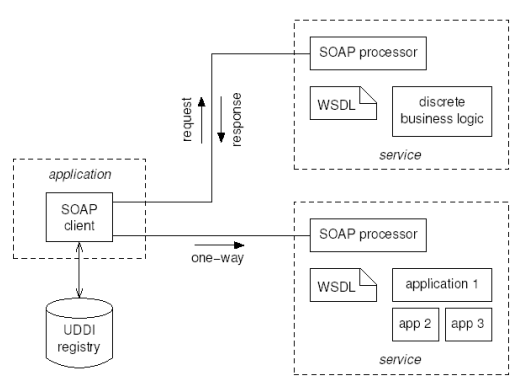
\includegraphics[scale=0.4]{figures/soap.png}
	\caption{Process of SOAP Message, from Client to Server and Back Again}
	\label{fig:soap}
\end{figure} 

\subsubsection{Message Format}

SOAP generally uses an XML based format. The message is contained in a SOAP envelope, which in turn contains a body and a header. The header contains instructions to the SOAP processor that receives the message, and the body contains the XML document which constitutes the payload of the request. Namespace declarations and encoding style directives are added to indicate that the request uses SOAP (and to specify the SOAP version). 

The \textbf{body} of the SOAP document represents the \textbf{requested method call}. The body should have a root element, indicating what the method is, and a series of either named or ordered sub elements which represent parameters to be passed to the method. The types specified for the arguments by the SOAP body must match up with the types on the actual method.

The \textbf{response} from the server is structured similarly. The root of the SOAP response body is conventionally the same as the the request, with `Response' appended. Sub elements represent one or many values returned from the method.

\begin{figure}[h]
	\centering
	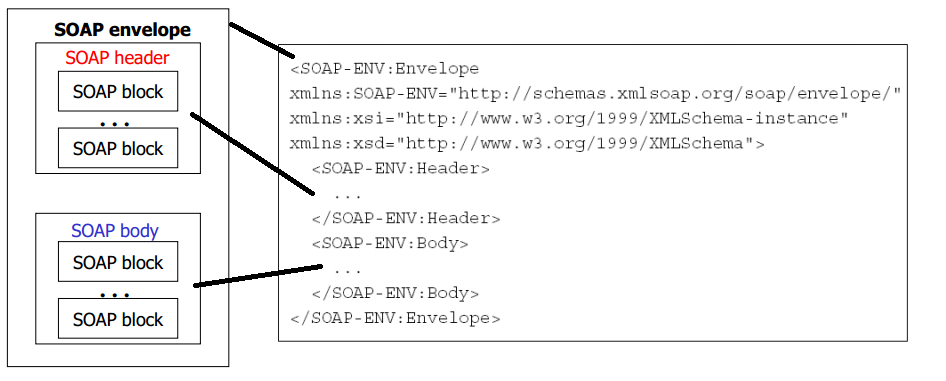
\includegraphics[scale=0.5]{figures/soap-envelope.png}
	\caption{SOAP Message Envelope Format, with Corresponding XML}
	\label{fig:soap-message-format}
\end{figure} 

\subsubsection{WSDL}

\textbf{WSDL (Web Services Description Language)} is a standard method of describing the interface of a web service using XML. It allows clients to recognize how to communicate with a web service automatically. It is a type Interface Description Language (IDL), similar to those used to describe the interface of a remote object. Whilst it allows clients to automatically determine how to communicate with the service, it adds \textbf{complexity to the web service}.

WSDL documents can often be auto-generated. The \texttt{Java2WSDL} tool generates a WSDL document for a compiled Java interface or class, and some SOAP containers such as \textbf{Apache Axis} will automatically generate WSDL documents if they're requested from the application code (such as a JAR file) that they are given. 

\subsubsection{Runtime Environment}

SOAP services typically use web server software to host the service, as \textbf{HTTP} tends to be the chosen method of transport. There are also custom implementations specialized for SOAP. Sun provide an implementation which is integrated into J2EE 1.4, and alternative implementations are provided by IBM, and the Open Source project Apache Axis. Microsoft provide support for SOAP services in the .NET framework. 

The \textbf{JAX-RPC} library is provided by Sun in order to communicate with existing SOAP services. An alternative is to use the \texttt{WSDL2Java} tool to generate a set of \textbf{stubs} from a service's WSDL document. These stubs act as an abstraction on top of the message passing system of SOAP, so that it appears to a developer to be like a normal method call (in the same way as RMI). If stubs are generated, the client becomes static (as it can't change its implementation), where if it parses WSDL documents and uses them to define how to call methods, the client can automatically adapt over time (with the server).


\subsection{REST}

\textbf{Representational State Transfer (REST)} is an alternative architectural style for web services. It originates from a 2000 PhD thesis by Roy Fielding. The driving principal of REST is that the standard protocols and principles of the web are sufficient for creating robust web services, so the additional complexity of SOAP is not needed. Whilst REST is \textbf{not a standard} in and of itself, it makes heavy use of the existing standards of the web. In particular, it is associated with HTTP, XML, JSON, URIs and sometimes HTML. 

At its core, REST is relatively simple. Application state and functionality is divided into \textbf{Resources} (for example, a person might be a resource). Each resource has a unique identifier through which it can be accessed (using a URI, typically a URL as defined in HTTP). A \textbf{constrained set of well-defined actions} can be performed on resources, as defined by the common HTTP verbs (GET, POST, PUT and DELETE), although some of these might not apply to all resources, or might be limited in some form (it might not make sense to delete some resources, or authentication and authorization might be required). The principals of REST do not specify any particular content-type for communication, but text based markups (primarily JSON and XML) are by far the most popular content types used.

As REST heavily utilizes the existing HTTP protocol (and other web protocols and technologies) it is several architectural properties common to the "traditional" web. It is a client-server model with layered protocols, which are almost entirely \textbf{stateless} and has caching support. In a well designed REST service, a resource can be retrieved in a fashion basically indistinguishable to how a web browser requests a document. 

A web page you'd retrieve via HTTP is a \textbf{resource}. So it is a JPEG picture file located on that web page. So are any links, sound files and soon. Resources are accessible using a \textbf{universal syntax} -- the URI. With REST, URIs are assigned:
\begin{itemize}
	\item individual data records
	\item pages
	\item remote procedures (\textbf{functionality})
	\item images
\end{itemize}
and so on.

\begin{figure}[h]
	\centering
	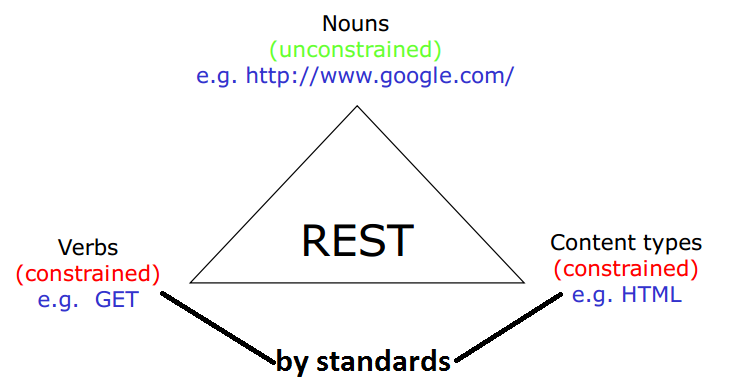
\includegraphics[scale=0.5]{figures/rest-triangle.png}
	\caption{REST Triangle. The verbs and content types are \textbf{constrained} because of the use of existing standards, but the nouns (services) are \textbf{unrestricted}.}
	\label{fig:rest-triangle}
\end{figure}

Resources are requested and modified through the standard HTTP verbs:
\begin{itemize}
    \item \textbf{GET} is the keyword primarily associated with retrieving content. It is analogous to READ in the CRUD acronym commonly used for databases.
    \item \textbf{POST} is often used to create resources, although it can be used to edit them. The primary difference between POST and PUT is impotence - POST is a non-idempotent action (i.e. calling the same method with POST twice can result in different responses). If there are different URLs (or payload formats) for editing and creating a resource, and a POST is sent to create a resource where it already exists, this could be considered an error. By returning 2 different results (create successfully if it exists, error if it doesn't) this request becomes non-idempotent. Likewise, if resources are created by sending a request to a `factory' URL (such as http://api.foo.com/myresource/) without the eventual URL of the resource being known (such as when IDs are auto incrementing, or when adding to a collection - http://api.foo.com/myresource/4) the action is also non-idempotent, as the same URL is being used in a request with different results (different resources being created). This would necessitate a POST. 
    \item \textbf{PUT} is typically used for editing a resource. Unlike a POST, PUT is idempotent, so no matter how many times the action is performed it will always have the same effect. This means that PUT requests can be retried or resent several times without causing unexpected behaviour (whilst this is not guaranteed with POST). It is often used to edit existing resources, as the resource which is sent will always replace any existing resource at that location (making it an idempotent action, as sending the same resource several times will have the same effect). PUT is also sometimes used to Create a resource, if the URL of the resource (subsequent to its creation) is already known (for example, PUTting to \texttt{http://api.foo.com/users/blah} would either create or update the user `blah' to make the resource at that address the same as the one sent in the request).
    \item \textbf{DELETE} is used for deleting a resource.
\end{itemize}
These operations are used to issue a request to a REST web service to \textbf{access and manipulate} the server-side state, or data record.

\paragraph{\textbf{NOTE: }} \textbf{CRUD} means Create, Read, Update, Delete.

Why is it called \textbf{Representation State Transfer}? Because:
\begin{enumerate}
	\item The client references a web resource using a URL
	\item A \textbf{representation} of the resource is returned (e.g. HTML document)
	\item The representation places the client application in a \textbf{state}
	\item The result of the client traversing a hyperlink in the document retrieves another document
	\item This new document is a \textbf{new representation} that places the client in \textbf{another state}. This new document has \textbf{transferred} the user from one state to another
\end{enumerate}

\subsubsection{Content Negotiation}

RESTful web services can return content in lots of forms. In order to determine which format the data should be returned in, clients can use the \textbf{Accept} header defined by the HTTP standard to define the acceptable return format. Valid values for the Accept header could be any MIME type, such as application/xml or application/json. Additionally, vendor specific MIME types can be used, which is often used for API versioning, or ensuring that responses conform to a custom schema.

Additionally, the c an specify what type of document they want using a \textbf{GET parameter}. Suppose you wanted to get a list of parts as an XML document, you may use the URL:
\begin{quote}
	\texttt{http:///www.parts-depot.com/parts?\textbf{flavour=xml}}
\end{quote}

Additionally, suppose you wanted an XML document for a specific part. You may use the URL:
\begin{quote}
	\texttt{http:///www.parts-depot.com/parts/23534}
\end{quote}
This is a \textbf{logical URL} which expresses what resource is desired. It is not a physical object/file. You don't need a million HTML pages if you have a million parts. It is possible to request and provide \textbf{virtual resources} what are accessed through a logical mapping of URL to resource (i.e. dynamically generate content).

\subsubsection{HATEOAS}

One of the key principals of REST is HATEOAS (Hypermedia As The Engine Of Application State). This defines a constraint on REST services that any client must interact with the service entirely through hypermedia generated by the service. This means that the client does not require any particular knowledge about a web service to interact with its contents, other than an understanding of hypermedia and an initial fixed URL of the service. This allows a client to navigate through the web service with little (or no) initial understanding of the resources, which provides a high level of decoupling between the client and the server, allowing them to evolve independently.

HATEOAS is an extension of the "Uniform Interface" constraint of the REST architecture.

Despite being one of the primary goals of the REST application architecture, HATEOAS is rarely implemented in commercial web services. 

\subsubsection{Resource vs Representation}

REST defines a distinction between a \textbf{Resource} and \textbf{Representations} of that resource. A resource is a conceptually entity usually present as part of the applications domain (for example, users or pets). A client communicates with the system by requesting and (perhaps to a lesser extent) performing modifications on \textbf{Representations} of a resource. For example, a service may have a concept of a user. A client could request a particular user object in XML, localized to German. It would be semantically the same as requesting the same object in JSON and French. They are simply different \textbf{representations} of the same \textbf{resource}.

\subsubsection{Advantages}

There are several proposed benefits of using REST as an application architecture.

\begin{itemize}
    \item \textbf{Improved Response Times} due to fundamental support for caching (by virtue of using HTTP) and the smaller size of requests (due to the lack of a SOAP envelope). SOAP messages cannot be cached as they always use POST (a non-idempotent action) for 8 all types of request (and the type is specified in the SOAP body). By contrast, REST systems can cache any idempotent operations (GET, PUT and DELETE - although usually only GET). Additionally, all resources of a SOAP service will use the \textbf{same URL}.
    \item \textbf{Improved Scalability} due to the lack of state (again because of HTTP), any server can handle any request, regardless of whether another server has handled a previous request from the same client. This greatly simplifies load balancing. 
    \item \textbf{Standards Compliant}. REST is based entirely on existing open standards and protocols which are well defined and understood (such as HTTP). This reduces the need to have vendor software or other mechanisms that layer additional messaging frameworks on top of existing standards (like SOAP, which is another framework on top of HTTP/SMTP/FTP/etc). That is, it \textbf{prevents vendor lock-in}.
    \item \textbf{Feature Parity} to alternative methods of communication (such as SOAP). This means it provides \textbf{equivalent functionality}.
    \item \textbf{No need for Resource Location} as HATEOAS makes it redundant. This simplifies the process of making a client. This is also provided through having a Generic Interface, which means that tools do not have to be customized per application (as they would have to be with SOAP). They merely need to understand the basic principals of HTTP. 
    \item \textbf{Compatibility/Evolvability} of services, as there is greater support for versioning. Different content types can be used to represent different representations, including different versions of the same representation (for example, HTML4 and HTML5). This also allows additional capabilities to be added to resources without breaking older clients (as newer representations can expose the new functionality).
    \item \textbf{Inspectability} of messages. REST interactions can be analysed much easier than SOAP messages, as the semantics of every SOAP application would have to be understood individually, whereas for REST only the principals and semantics of HTTP need to be known. This makes it easier to implement proxy servers or gateways which filter out certain types of interactions. 
\end{itemize}

REST is currently growing in popularity amongst those requiring web services, partly due to its ease of implementation. Many companies are using it to expose their data and allow integration with their applications and platforms. REST is often considered to be faster than SOAP (with Amazon quoting their REST services being up to 6 times faster), and more popular (with around 80\% of Amazon's clients opting to use the REST interface over SOAP).

SOAP is typically used to integrate internal systems, or larger, more complex applications which require a \textbf{higher degree of formality} in their communications. SOAP can have richer functionality, but it comes at the expense of interoperability with other systems. Therefore, SOAP is good for DSes that required advanced capabilities between relatively homogeneous systems. 

\subsubsection{Java and REST}

Java implements REST support via the Java Specification Request (JSR) 311 (otherwise known as JAX-RS). JAX-RS uses annotations to define how classes are relevant to REST. Either XML or JSON can be used via JAXB (Java Architecture for XML Binding).

The reference implementation of JAX-RS is \textbf{Jersey}, which provides both a REST client and server. It uses a scanner to identify REST resources (using reflection?) and expose them using a servlet. A \textbf{ Web Application Description Language (WADL)} document is generated (which is similar to a WSDL) and automatically exposed by the servlet. 


\section{Naming}

In order to get access to a resource, they must be \textbf{named}. Whether that resource is a computer, printer, document or web page, it must be identifiable by a name of some form. Names could be human readable, or might be a string of bits or characters. 

A name represents a series of \textbf{attributes} of an entity. \textbf{One} of these attributes will typically give access to the entity. Changing a name into its related attributes is known as \textbf{resolving} the name. Figure \ref{fig:name-resolution} shows the archetypal example of a name resolution system, the WWW. Notice how the URL specifies different components of the resource's name, all of which are resolved to retrieve the final file.

\begin{figure}
	\centering
	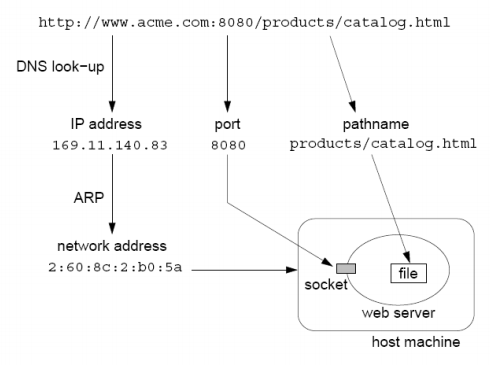
\includegraphics[scale=0.6]{figures/naming-resolution-example.png}
	\caption{An Example Resolving Name to Exact Resource (DNS)}
	\label{fig:name-resolution}
\end{figure}

\textbf{Access Points} are ways of actually operating on an entity or resource. The name of an access point is usually referred to as its \textbf{address}, which is also usually thought of as the address of the entity itself. A resource can have \textbf{several access points} (e.g. URL redirection), and they can change over time. Because of this, a \textbf{location-independent} name is usually chosen for resources.

\subsection{Naming Services}

The responsibility of a \textbf{naming service} is to manage the relationship between resources and attributes, primarily translating the name of a resource into its attributes (performing \textbf{name resolution}). It is also responsible for creating, deleting and listing the bindings between resources and attributes, and organizing the the collection of valid names recognized by the service. This collection is known as the \textbf{namespace}.

\subsubsection{Namespaces}

The namespace is the collection of valid names recognized by the service. They can either be flat or hierarchical. 

\textbf{Flat namespaces} are usually finite in length, as the size of the names is usually limited. For example, if names were based on 32-bit integers, there could only be $2^{32} = 2,147,482,65$ items in the namespace. 

\textbf{Hierarchial namespaces} can grow indefinitely as each part of a name is resolved \textbf{relative to parent elements}, so name fragments can be \textbf{reused} across different components. The different contexts (subtrees formed from children) can be managed by different individuals too, aiding administration of large namespaces. A hierarchical namespace can be visualized as a graph with leaf nodes and "directory" nodes. Leaf nodes store the actual entity attributes, where directory nodes are used to navigate to the appropriate leaf.

Common examples of a hierarchical namespace would be a \textbf{file system or DNS}. A file system has directory nodes (actual directories, or folders), which are used to allow multiple documents to have the same name and to help navigate to a document, and leaf nodes (the actual documents), which store the contents. A file system also shows that a hierarchical namespace graph does not have to be a tree -- \textbf{symbolic links} can be used to reference the same document from multiple directories (resulting in cycles).

\begin{figure}[h]
	\centering
	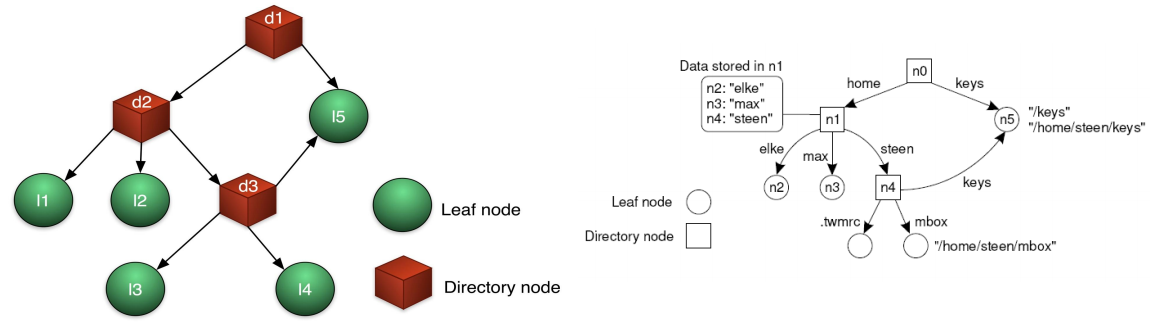
\includegraphics[scale=0.5]{figures/naming-filesystem.png}
	\caption{Operating System Filesystems are Examples of Hierarchial Naming Systems}
	\label{fig:filesystem-naming}
\end{figure}

In order to find nodes, an \textbf{initial starting point} must be known. In a file system, this is traditionally the first inode of a logical disk (which can in turn be calculated by information from the disks superblock). In other systems, some starting point must be defined (like a \textbf{name server address} in DNS).

Hierarchical namespacing is a much more scalable technique. It allows an infinite number of names to be stored (as you can merely add layers to the graph) and allows different parts of the graph to be administrated by different people. By partitioning the graph, and allowing parts of it to be replicated (caching close to points of need) the system can be very scalable and resilient. These properties are perhaps best shown in DNS. Name servers contain attribute data for the names in their domain, and also hold references to other name servers (authoritative name servers for delegated sub domains - children, and at least 2 servers with authoritative data for the zone - parents). Any name server can replicate information from another, as long as it informs its clients that the name record is not authoritative (i.e. it is replicated, and therefore may be inconsistent), and that it stores a time to live after which it will contact the authoritative name server to verify the data is still correct. 

If the name database or number of users is very large, we cannot store all naming information on a \textbf{single service machine}. \textbf{Replication} of the database and \textbf{caching} of the results of name resolution are essential to meet performance and reliability of targets. Resolution is also quicker if the namespace is structured hierarchically -- this also makes replication easier. This makes hierarchial namespaces much more \textbf{scalable}.

This is known as \textbf{distributed naming}, which is something DNS performs. Section \ref{sec:dns-lookup} uses DNS as an example of distributed naming and the concerns you need to think about.

\subsection{Example Naming Service -- DNS}
\label{sec:dns}

\begin{figure}[h]
	\centering
	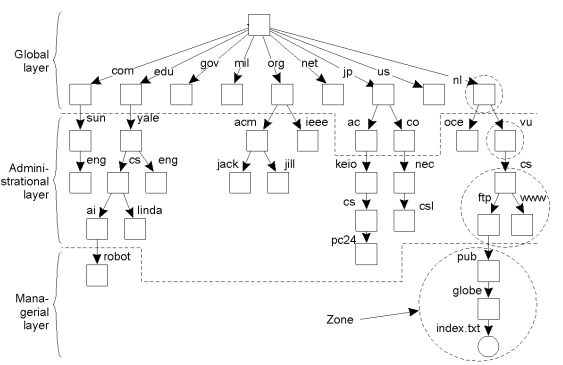
\includegraphics[scale=0.7]{figures/dns-graph.png}
	\caption{DNS Naming System's Graph (Multiple Layers)}
	\label{fig:dns-graph}
\end{figure}

A naming service is used to look up entities based on their names. The most prominent example of a directory service is DNS. DNS is a \textbf{traditional naming service}. You give it a name and it resolves the name to a node (which contains an IP address among other things) in the \textbf{naming graph}, returning said node. Conceptually it is equivalent to a person using a telephone directory (they give a name and get a telephone number).

Examples of \subsubsection {DNS Resource Records} include:
\begin{itemize}
    \item \textbf{SOA} (Start of Authority record) used for zone parameters
    \item \textbf{NS} (Authoritative Name Server) used for domain names
    \item \textbf{A} (Computer Address) used for IP Addresses
    \item \textbf{CNAME} (Canonical Name) The canonical domain name for an alias
    \item \textbf{MX} (Mail Exchange) Information for mail exchange (Email), such as preferences and the hostname
    \item \textbf{HINFO} (Hosting Information) Hosting information for this node (such as architecture and OS)
    \item \textbf{TXT} (Text) Arbitrary text information
\end{itemize}
This information is stored at each node in the naming graph.

Another approach is to store a \textbf{description} at a node and then use \textbf{partial descriptions} to retrieve (possibly multiple nodes). This is similar to a search query in information retrieval or \textbf{content-addressable memory}. This is known as a \textbf{directory service}.

\subsubsection{DNS Zones}

The hierarchical DNS database is split into 3 zones. The \textbf{Global} zone is the highest level (responsible for .com, .edu, etc) and is worldwide. There are a small number of nodes at the global level, which means they may take a matter of \textbf{seconds} to respond to requests. This is combated by having a high level of replicas lower down the chain. Updates are propagated lazily though the graph (only updated when node is accessed again).

The second level is the \textbf{Administrative} zone. It takes place on an organizational basis (i.e. .yale.edu, .microsoft.com, etc.). There are a much \textbf{higher number of nodes} at this level, which makes it comparatively faster to look up (in the scale of milliseconds). Updates are immediately propagated and there usually aren't many replicas (if any at all).

Finally, there is the \textbf{Managerial} zone, which is geographically appropriate to a department. There are millions of managerial nodes worldwide, and they therefore don't tend to have replicas. They can however, respond to a lookup immediately. They also don't \textit{always} apply client-side caching, where both of the higher tiers do. This is because this zone is \textbf{constantly changing}, as it is the layer where all the web pages, services and so on reside.

\subsubsection{DNS Lookup}
\label{sec:dns-lookup}

DNS Lookup can be \textbf{Iterative}, \textbf{Recursive} or \textbf{Multicast}.

\textbf{Iterative} resolution relies on the client going to the root server and requesting a single child node, making a requests to the child for the next child, and so on. It iteratively requests the nnext child the process until it reaches the correct node (a leaf). For example, in \textbf{leeds.ac.uk}, the root server would be consulted which would return the .uk server. The .uk server would return the .ac and the .ac would return the .leeds node. The key behind this is that the \textbf{client} is requesting from each name server, as shown in Figure \ref{fig:dns-iterative-lookup}. In this example, the client has to make 4 calls over a WAN, which is very slow.

\begin{figure}[h]
	\centering
	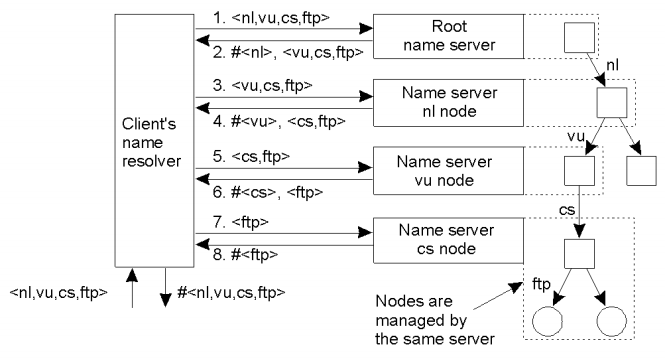
\includegraphics[scale=0.6]{figures/dns-iterative-resolution.png}
	\caption{Iterative Name Resolution with DNS}
	\label{fig:dns-iterative-lookup}
\end{figure}

\textbf{Recursive} resolution relies upon the first server directly asking the second server, and so on and so forth (rather than simply pointing the client and telling it to ask). The original name server will then respond to the clients request directly (so there is only one request \textbf{visible to the client}. Recursive name resolution places greater demand on the name server, so some name servers with particularly high throughput may not support it (for example, in the global layer). However, in a recursive solution the name servers can \textbf{cache addresses}, gradually learning about more name servers which handle lower-level nodes and passing this benefit on from that point onwards. In an iterative resolution approach, only the clients name resolver gets the benefit of the cache (and other clients won't). A recursive approach may also reduce the communication overhead, depending on the overhead between name servers. This is because they will probably have better connections and less latency between each other than between a client and name server (perhaps due to being geographically close). In Figure \ref{fig:dns-recursive-lookup}, the client only makes a single  WAN call, with the requests between name servers being shorter communication.

\begin{figure}[h]
	\centering
	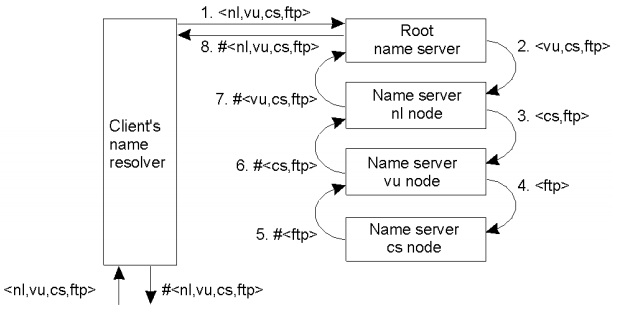
\includegraphics[scale=0.6]{figures/dns-recursive-resolution.png}
	\caption{Recursive Name Resolution with DNS}
	\label{fig:dns-recursive-lookup}
\end{figure}

\textbf{Multicast} resolution requires the name to be broadcast to \textbf{all name servers}, and the one that is holding the binding for the name responds. An additional server is required, to handle what happens if a name is not bound. 

The communication costs of iteration and recursive lookup are shown in Figure \ref{fig:dns-lookup-costs}. Iterative resolution has more WAN, long-distance communication than recursive resolution. This may make it slower to resolve.

\begin{figure}
	\centering
	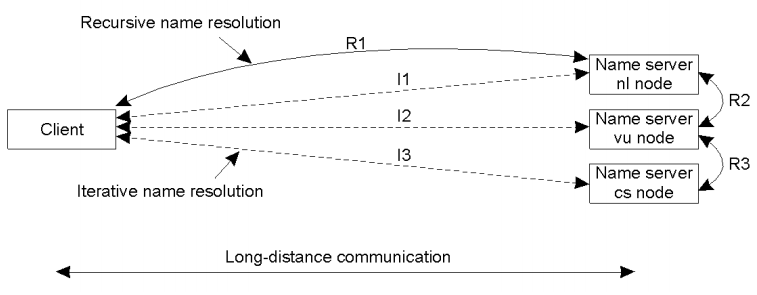
\includegraphics[scale=0.6]{figures/dns-lookup-costs.png}
	\caption{Illustration of Communication Required (thus, the cost required) to Perform Iterative and Recursive DNS Lookup}
	\label{fig:dns-lookup-costs}
\end{figure}

\section{Directory \& Discovery Services}

Directory and Discovery Services are used to find entities within a graph. They offer alternative approaches for performing the same action - a \textbf{directory} service looks up a resource by its name or other attributes, where a \textbf{discovery} service finds a resource which matches some specification. 

\subsection{Directory Service}

A \textbf{directory service} is an alternative to a naming service. Rather than resolving a node in the graph from its name, a \textbf{description} is stored at a node, and a \textbf{partial description} can be used to retrieve a node (and possibly similar nodes). It is conceptually similar to using the Yellow Pages (give me the phone number for a plumber) rather than using a telephone book (give me the phone number for John Smith). This works similarly to content-addressable memory or information retrieval.

It can be regarded as the opposite of a naming service, as it allows an entity to be looked up by it s description (or properties) as opposed to name. It is useful for when a client needs a service, but doesn't really care what actual entity provides it.

\subsubsection{X.500}

\textbf{X.500} is part of the Open Systems Interconnection (OPI) set of standards. It is popular due to lightweight implementations created as Internet services. Data is organized into named nodes in a tree structure (the Directory Information Tree, or DIT). The entire structure, \textbf{including the data} contained within the nodes is known as the Directory Information Base (DIB). The aim of the system is to have a \textbf{globally unique name} for each leaf node, which has lead to a global DIB distributed across many servers (like DNS). 

The primary difference with X.500 and DNS is that X.500 is query-able. For example, it would be possible to search for all departments in the University of Leeds. However, searching is generally expensive as it may need to access several leaf nodes and combine results. An example of a query would be \begin{quote}\texttt{search("\&(C=GB)(O=University of Leeds)(OU=*)"})\end{quote}.

Table \ref{tab:x500} shows some of the \textbf{naming conventions} used for the X.500 namespace. The first five are commonly used, whereas the last two are dependant on the organisation/department.

\begin{table}
	\centering
	\begin{tabular}{|l|l|l|}
		\hline
		\textbf{Attribute} & \textbf{Abbr.} & \textbf{Value} \\
		\hline
		Country & C & GB \\
		Locality & L & Leeds \\
		Organization & OC & University of Leeds \\
		OrganizationalUnit & OU & School of Computing \\
		CommonName & CN & Roger Boyle \\
		EmailAddress & & roger@comp.leeds.ac.uk \\
		RoomNumber & -- & 8.03c \\
		\hline
	\end{tabular}
	\caption{X.500 Namespace}
	\label{tab:x500}
\end{table}

\subsubsection{LDAP}

\textbf{LDAP (Lightweight Directory Access Protocol)} is an alternative to X.500 and its Directory Access Protocol. Where X.500 (and the associated protocol) is complex and difficult to use, LDAP is implemented on top of TCP, which provides a much simpler interface for accessing X.500 services. It is now seen as the standard for Internet based directory services (for example, Microsoft's Active Directory has an LDAP interface). 

\subsection{Discovery Services}

How can businesses find out what web services are exposed by their potential partners? How can developes find the \textbf{WSDL} data they need in order to implement a client for a particular service? How can software that wishes to invoke a \textbf{specific service} determine whether that service is implemented in a compatible way.

A \textbf{discovery service} addresses all of these problems. Developers \textbf{register} their services and \textbf{users} search for services  that meet their requirements using SOAP (or REST.

\subsubsection{UDDI}

\textbf{UDDI (Universal Discovery, Description and Integration)} is a solution to the problem of finding web services. It is a discovery service which provides WSDL data for web services in response to requests from clients. It allows clients to find web services which implement certain functionality, and are compatible with them. 

The service provider creates a UDDI \textbf{business registration} (which is XML) and publishes it. These business registrations are stored in a UDDI Business Registry, which is \textbf{replicated} throughout UDDI Operator Sites. The registry itself is a web service, so it can be communicated with using SOAP over HTTP. Relevant messages can be constructed or parsed by calls to an \textbf{inquiry API} and a \textbf{publishing API}. There are several implementations of UDDI, including for .NET (UDDI.NET) and Java (jUDDI). 

\subsubsection{Spontaneous Networking Environments}

In a \textbf{spontaneous networking environment}, clients can connect without warning, and without preparation (by administrators). The services available are also spontaneous, and may disappear and appear without warning. In order to deal with this unreliable environment, there must be support for \textbf{automatic registration and de-registration of services}, and the discovery of available services by a client. Spontaneous networking environments are one of the perceived problems of distributed systems, and there are various solutions to these problems. Jini (or Apache River) is a networking architecture developed by Sun which allows for modular services co-operating services to be used to construct a distributed system.

\subsection{Java Naming and Directory Interface (JNDI)}

JNDI is an API for directory services that allows clients to \textbf{discover and lookup data and objects via a name}. JNDI is independent of the underlying implement, meaning it could be used for Internet resources (DNS), file systems, flat files or databases.

The API provides:
\begin{itemize}
	\item a mechanism to \textbf{bind} an object to a name
	\item a directory lookup interface that allows \textbf{general queries}
	\item an event interface that allows clients to determine when directory entries have been \textbf{modified}, meaning caching can be implemented
\end{itemize}
Examples of frameworks that use JNDI is the RMI registry (flat) and the file system (hierarchical).

Functionality for JNDI is implemented in \textit{javax.naming} (especially in the \textit{Context} interface and \textit{InitialContext} class). The starting location for a lookup is the \textit{InitialContext} class, which has a \textit{lookup} method allowing for objects (including sub-contexts) to be looked up by name. An object can be added to a context by the \textit{bind} method. LDAP also uses the JNDI API.

\section{Timing and Synchronization}

One of the major problems of distributed computing is that there is no centralized, globally agreed upon time. Where in a centralized system, the current time is unambiguous (not necessarily correct, but consistent), this assumption \textbf{does not hold} in a distributed environment. There is \textbf{no global agreement} on time.

\subsection{Time Standards}

The current standard for time was defined in 1958 as the time it takes for caesium 133 atom to make 9,192,630,770 electronic transitions (prior to 1958 and the invention of the atomic clock, mean solar seconds were used). 50 laboratories around the world measure the number of atomic clock ticks since the 1st of January 1958, and this is averaged to produce the International Atomic Time. As the mean solar day is getting longer, leap seconds are introduced to recalibrate the time (so noon does not get earlier). This occurs whenever there is a discrepancy of 800 ms between atomic and solar time.

The time based on TAI (atomic time) and including leap seconds is called \textbf{Universal Coordinated Time (UTC)}. UTC synchronization is performed via satellite or radio transmission.

\subsection{Drift}

Every machine has an internal physical clock, which uses a quartz crystal to measure the time. Each crystal oscillation decrements a counter, and when it hits 0 a timer interrupt (a clock tick) is generated, and the counter is reloaded. Battery powered RAM stores the number of clock ticks since a known point (an \textbf{epoch}), so the system can determine the date and time. However, crystals will run at different rates, causing clock skew between different machines.

At UTC time $t$, the value of the $i$th clock in the system is $C_i{t}$. Ideally, $C_i(t)) = t + \gamma$ for all $i$ and $t$, and $\frac{\Delta C}{\Delta t} = 1$. In other words, the \textbf{drift} of every clock in the system is the \textbf{same}, and the clock's value is changing at the same rate (and at the same time) as the actual time $t$ (a clock should tick when a second actually goes by).

\begin{equation}
\begin{aligned}[b]
	\frac{\Delta C}{\Delta t} > 1
	\;\;\;\;\;\; \text{fast clock} \\
	\frac{\Delta C}{\Delta t} < 1
	\;\;\;\;\;\; \text{slow clock} \\
	\frac{\Delta C}{\Delta t} = 1
	\;\;\;\;\;\; \text{perfect clock} \\
\end{aligned}
\end{equation}

If we set a \textbf{maximum allowed drift rate} $p$, we consider a time as \textbf{working properly} if:
\begin{equation}
	1 - p \leq \frac{\Delta C}{\Delta t} \leq 1 + p
\end{equation}
where $0 \leq p \leq 1$. Currently, clocks are generally accurate to within $10^{-5}$ of the actual time, so $p = 10^{5}$ would be a good maximum drift rate.

By imposing a maximum drift rate $p$, two clocks may as far as $2p\Delta t$ apart. This occurs because both clocks may be drifting away from UTC at a maximum of $p$, but in \textbf{opposite directions} (one moving fast, one moving slow).

\begin{figure}[h]
	\centering
	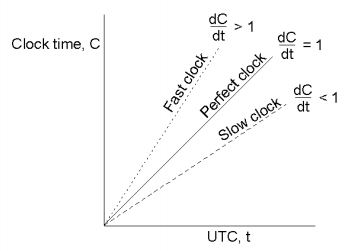
\includegraphics[scale=0.6]{figures/utc-drift.png}
	\caption{Visualisation of UTC Drift Measurement}
	\label{fig:utc-drift}
\end{figure}

By having a maximum drift rate ($p$), 2 clocks within a distributed system can be guaranteed to be within $2p \theta t$ at time $T$. This occurs because both clocks may be drifting away from UTC at a maximum of $p$, but in opposite directions (one moving fast, one moving slowly). This is shown in Figure \ref{fig:utc-drift}.

\subsection{Christian's Algorithm}

\textbf{Christian's algorithm} presents a way to solve timing and synchronization issues by using a \textbf{centralized UTC server}. A machine with a UTC receiver is deemed the \textbf{time server}. Every machine sends a message periodically (interval between messages not exceeding $\frac{\Delta}{2p}$ seconds) to the time server, requesting the current canonical time. The server responds as quickly as possible with the current time according to UTC $C_{UTC}$. 

This introduces two major problems. The first is clocks that may be running quick. If they adjust to use the canonical time immediately, it would appear to applications as though the system has \textbf{gone back in time}. This may cause issues, such as resources being deleted before being created in audit trails. In order to deal with this, a fast client must adjust its time to $C_{UTC}$ \textbf{gradually}. This problem does not affect slow clients, as they can merely "skip" a few seconds. 

The second major issue is \textbf{network latency}. The message containing the current UTC time will never arrive instantaneously, and will therefore be incorrect when it arrives at the client. It will be more incorrect the bigger the network latency. One method of estimating the amount of time it has taken for the message to arrive is to measure the \textbf{time between request and response and to divide it by 2}, to approximate the cost of the message going in one direction. You would then subtract this computed time from the received time. Figure \ref{fig:propagation-time} illustrates the network latency. We can take this into account and compute the \textbf{time of clock $i$} like so:

\begin{equation}
	C_i(t) = C_{UTC} - \frac{t_1 - t_0 - I}{2}
\end{equation}

\begin{figure}
	\centering
	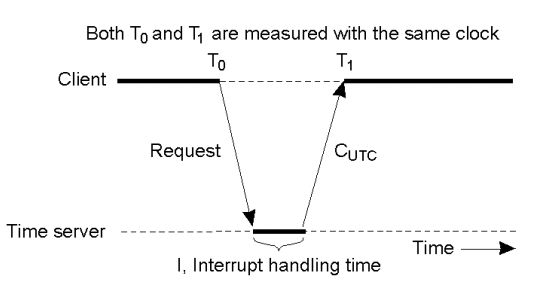
\includegraphics[scale=0.6]{figures/propagation-time.png}
	\caption{Computing Time it Took Real UTC Time to Propagate (Arrive) at a Server}
	\label{fig:propagation-time}
\end{figure}

\subsection{Berkeley Algorithm}

In the \textbf{Berkeley algorithm}, there is a \textbf{time daemon} which asks all of the machines in the system what the time is according to their internal clocks. All of the machines in the system answer, and the time daemon informs all of its clients how to adjust their clocks. This is a useful technique for when a UTC reference point is not present. The Berkeley algorithm will simply \textbf{average the clocks} of the clients to determine the correct canonical time within the system.

It is used to \textbf{minimise time differences} when there is no central UTC receiver to work from.

\begin{figure}
	\centering
	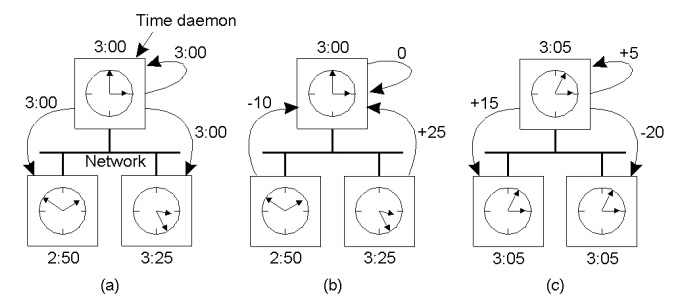
\includegraphics[scale=0.5]{figures/berkeley-algorithm.png}
	\caption{A Time Daemon Synchronising all the Clocks in the System using the Berkeley Algorithm}
	\label{fig:time-berkeley}
\end{figure}

Figure \ref{fig:time-berkeley} shows an example of the Berkeley algorithm running on a DS. The time daemon computes the average of all three times (including the \textbf{time daemons}) and then sets every clock in the system to that average (this again includes the time daemon!)

\subsection{Network Time Protocol}

In order to send timing information over the Internet, \textbf{NTP (Network Time Protocol} is used. Christian's and Berkley Algorithms are not suitable to the Internet, as they require either a centralized daemon or time server. It provides a reliable service which can survive losses of connectivity, and provides an authentication layer to prevent interference with the service (malicious or otherwise). Clients can resynchronize frequently enough to offset common drift rates.

In order to maintain scale, NTP forms a logical hierarchy called a \textbf{synchronization subnet}. Primary servers, those in \textbf{stratum 1}, are connected directly to the time source (the UTC reference point). Secondary servers synchronize with those in stratum 1, and so forth. Leaf nodes are individual users workstations. The accuracy of the time decreases proportionally to the layer of the strata (the bottom layer having the least accurate time). 

NTP is the time-equivalent of DNS. It is a highly robust service, which has been widely deployed throughout the Internet for a number of years. It is generally recognized as the best in class solution for unreliable networks, providing accurate timing information to within a few milliseconds over the Internet, or within sub-milliseconds on local networks.

\begin{figure}[h]
	\centering
	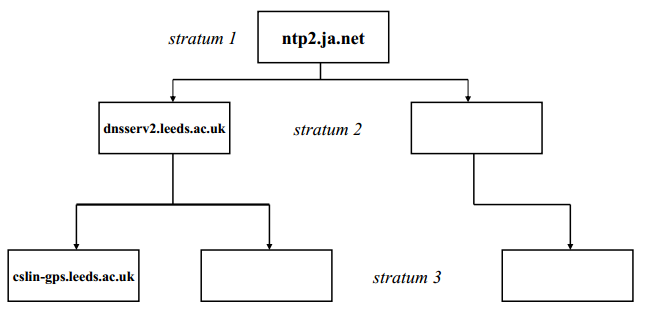
\includegraphics[scale=0.5]{figures/ntp.png}
	\caption{Hierarchical Architecture of Servers using NTP. Accuracy of time decreases as we move down the strata, with the roots (stratum 1) being servers that directly receive time from satellites.}
	\label{fig:ntp}
\end{figure}

\section{Current Trends}

Over time, several trends have emerged in distributed systems. These are often driven by enterprises, which seeks to integrate disparate systems together (to provide business value), manage ever-complex IT systems (databases, Operating Systems, networks, storage, new application development) and to plan for new vendor techniques and technologies.

\subsection{On-Demand Computing}

On-Demand computing is becoming a popular model in response to the challenges of enterprise IT. Computer resources are acquired and used on an \textbf{on-demand basis}. When computer resources are needed, they are utilized and when they are not they are discarded. 

If an enterprise plans for its \textbf{peak requirements}, they may end up paying a large amount for computer resources that they don't need the majority of the time. However, if they only purchase the minimum resources, they will face problems when they reach the peak of their utilization (as they will have inefficient resources to deal with the work load). For example, an online shop might use several times the amount of computing resources around Christmas time. They don't need that level of resources any other time in the year, so purchasing that amount of infrastructure would be a waste of money for the rest of the year. However, without those resources they cannot capitalize on the Christmas rush. The flexibility of \textbf{On-Demand Computing} is crucial in meeting these fluctuations in demand.

\subsection{Utility Computing}

The concept behind utility computing is to provide a service whereby organizations \textbf{outsource} their demand for computer resources to other companies, who act as external service providers. The resources that they use from the external service providers are paid for on a \textbf{per-usage basis}. Customers access their computing resources over a network (typically the Internet, but it could be a private network) and pay for the length of computing time that they use. 

This is analogous to other common utilities, such as gas or electricity. Electricity, for example, is acquired from power companies (service providers) and sent through the power grid (similar to the Internet). The customer pays for how much electricity they use (as opposed to a one off, or constant cost payment) and can scale their usage of power up and down as required (for example, more in winter but less when they're on holiday abroad).

\section{Grid Computing}
 
\textbf{Grid Computing} is a type of utility computing. Grids are typically geographically diverse networks consisting of a (potentially) large number of \textbf{commodity computing resources}, connected together to provide unlimited storage and computing capacity. The Grid aims to facilitate the sharing of \textbf{everything} (where the Web aims to facilitate the sharing of information). 

The main problem that Grids attempt to solve is the sharing of computer resources between dynamic collections of individuals, organizations and institutions. These communities (or \textbf{virtual organizations}) can share computing resources as they pursue common goals. An example of this is the \textbf{White Rose Grid}, which the University of Leeds, University of York and University of Sheffield often use to collaborate on shared projects.

\begin{figure}[h]
	\centering
	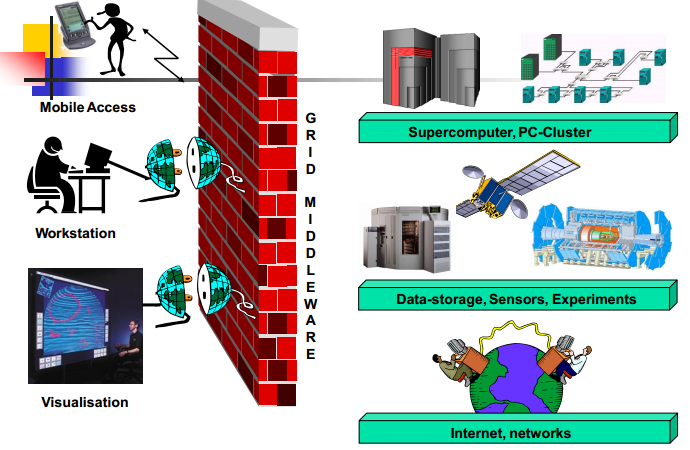
\includegraphics[scale=0.5]{figures/grid.png}
	\caption{Grid computing is analogous to the electricity grid. You just tap into the grid and receive access to the desired resources (which can be \textit{anything}).}
	\label{fig:grid-computing-analogy}
\end{figure}

The concept of a grid has transformed research, business, medicine and engineering. According to Ian Foster, there are \textbf{three major requirements for a grid system}:
\begin{itemize}
    \item \textbf{Co-ordination of resources that are beyond central control} -- so there is no single entity saying "I'm controlling the grid.". This involves authentication, authorization, accounting (auditing) and distributed algorithms.
    \item \textbf{Standard, Open, General-purpose protocols and interfaces} -- reuse as much as you can/ This relies on standard and open protocols for all machines to communicate easily (makes adding new machines to grid and \textbf{scaling} it more easier)
    \item \textbf{Non-Trivial Quality of Service}--  including the guaranteed ability of remote access, resource management, fault management (and tolerance), guarantees of performance and monitoring.
\end{itemize}

\subsection{Layered Grid Architecture}

Figure \ref{fig:layered-grid-architecture} shows the \textbf{layered} architecture of the grid; this is analogous to the Internet architecture 5 or 7 layer). The layers are as follows:
\begin{itemize}
	\item \textbf{Application} -- Where the applications that run on the grid reise
	\item \textbf{Collection} -- coordinates multiple resources, infrastructure services. Includes co-allocation, scheduling and directory services monitoring.
	\item \textbf{Resource} -- Sharing single resources, negotiating access of said resources and controlling their use. Includes configuration, current load on resource and usage policy (is host $x$ allowed to use service $y$ this much or on this date?)
	\item \textbf{Connectivity} -- about "talking to things". Deals with communication and security through Internet protocols, single sign-on and trust relationships. This encapsulates the \textbf{Transport and IP layers} of the Internet layered architecture
	\item \textbf{Fabric} -- about controlling things locally. Controls access to, and control of, \textbf{computational and storage resources}, catalogues and networks
\end{itemize}

\begin{figure}
	\centering
	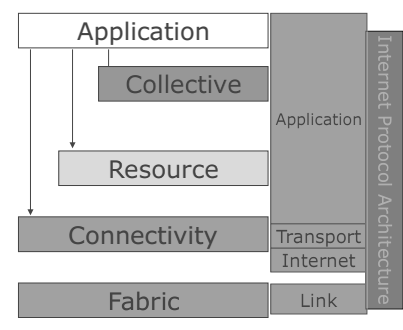
\includegraphics[scale=0.5]{figures/grid-layered-architecture.png}
	\caption{Layered Grid Architecture}
	\label{fig:layered-grid-architecture}
\end{figure}

\subsection{Open Grid Services Architecture}

The \textbf{Open Grid Services Architecture (or OGSA)} is motivated by the need to integrate \textbf{services} (not just computing power) across distributed virtual organizations, all with different platforms and technologies (heterogeneous). It is designed to focus on the nature of the services in the grid, that respond to particular messages. In other words, it is a way of seeing the grid as a \textbf{extensible set of services}.

This vision can be combined with web services to inherit many of their advantages, such as service description and discovery. Pretty much \textbf{everything} becomes a service. However, grid services (and web services in general) tend to provide clients with the ability to view and modify the state of entities (resources). Whilst services are usually designed in this manner (despite the stateless nature of HTTP), there is no \textbf{explicit} interface indicating that the service is \textbf{stateful}. In other words, web services are stateless unless explicitly stated -- but how does a grid know this? See Figure \ref{fig:stateless-stateful-web-invocation} for an illustration of stateless web services and the stateful equivalent.

\begin{figure}
	\centering
	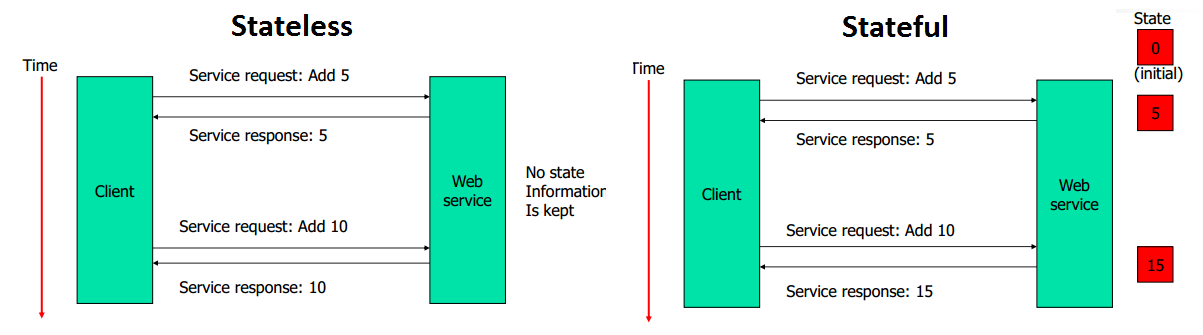
\includegraphics[scale=0.5]{figures/stateless-stateful-services.png}
	\caption{Stateless and Staeful Service Invokation over Web (HTTP)}
	\label{fig:stateless-stateful-web-invocation}
\end{figure}

The \textbf{Web Service Resource Framework (WSRF)} is designed to solve this issue. WSRF is a set of 5 technical specifications, defined in terms of message exchanges and XML definitions. It allows web service resources to be declared, created, accessed, monitored or observed for change, and destroyed via conventional web service mechanisms.  WSRF acts as an \textbf{extension} of \textit{conventional} web services. OGSA \textbf{requires} WSRF to be in place.

\subsection{Technical Challenges}

There are various challenges associated with grid computing:
\begin{itemize}
	\item \textbf{Security and Trust} is a persistent problem, as there is no central control over a grid, due to the fact it spans across \textbf{multiple} administrative domains, and possibly across nationalities (all parties and machines should trust each other).
	\item \textbf{Resource Stability} is also an issue, as the characteristics of resources can change over time and location. That is, resources/services enter the grid and then leave again.
	\item \textbf{Complex Distributed Applications} are a natural fit for the grid, and come with complex requirements for resource allocation and complicated work-flows.
	\item \textbf{Guaranteed performance} in a situation which is always changing, with heterogeneous platforms. Each machine may have different middleware, different specifications and so on -- this should not matter! This also means the grid must also be fault tolerant and handle broken down machines.
	\item \textbf{Virtualisation} of resources.
\end{itemize}


\section{Cloud Computing}

Cloud Computing has become a major trend in distributed systems, offering on-demand, utility computing. A combination of servers, connections, software and services are made available over the Internet in a \textbf{(fairly) transparent} manner. This network is known as \textbf{"the cloud"}. Having access to the cloud allows users to have a great amount of computing power from the most basic devices known as \textbf{"thin clients"}. (such as mobile devices or "dumb" terminals). It also lets organizations scale their computing resources according to demand.

The \textbf{primary differences} between the Grid and the Cloud are that the cloud is usually \textbf{centralised} (having one supplier, such as Amazon) where the Grid is decentralized. Additionally, the cloud offers on-demand services (pay for what you use), whereas this is \textit{not} one of the priorities of the Grid.

Technology companies are increasingly embracing the \textbf{Service Orientated Economy}. They are increasingly outsourcing parts of their technology stack (for example, using Salesforce) to reduce complexity and cost. This leads to the requirement of Service Orientated Infrastructure to cope with this new demand. This infrastructure needs to facilitate the deployment and management of services.

\subsection{Definitions}

There are various definitions of Cloud Computing.

It can be seen as an information technology infrastructure in which computing resources are \textbf{virtualised and access as a service}. Clouds are \textbf{large pools} of easily usable and accessible virtualised resources. Resources can be \textbf{dynamically reconfigured} to adjust to a variable load (\textbf{scale}), allowing also for an optimum resource utilisation (\textbf{elasticity}). This pool of resources is typically exploited by a pay-per-use model in which guarantees are offered by the infrastructure provider by means of customized \textbf{Service Level Agreements}.

What do cloud service consumers what? They want to \textbf{minimise expenses and meet quality of service agreements}. They may ask the following questions;
\begin{itemize}
	\item how do express QoS requirements to meet my goals? (computation/storage requirements)
	\item how do I assign valuation to my application?
	\item how do I discover services and map applications to meet QoS needs? (e.g. are they in a registry?)
	\item how do I manage multiple providers and get my work done?
\end{itemize}

What do cloud service providers want? They want to \textbf{maximise profit and attract customers}. They may ask the following questions;
\begin{itemize}
	\item how do I decide service pricing models?
	\item how do I specify prices?
	\item how do I translate prices into resource allocations?
	\item how do I assign and enforce resource allocations?
	\item how do I advertise and attract consumers?
	\item how do I perform accounting?
\end{itemize}

\subsection{Providers}

There are several providers of Cloud Computing. Amazon EC2 (Elastic Compute Cloud) is one such service which allows a resizeable amount of computation capacity. It allows for new capacity to be obtained on demand with little friction, and reduces the amount of time taken to acquire, provision and boot servers significantly, allowing capacity to be scaled very quickly (providing true on-demand computing). 

There are several alternative Cloud Computing providers such as Microsoft Windows Azure and Rackspace. 

Cloud providers will typically have \textbf{10s to 100s of thousands of physical machines}, usually together in data centres. This means that cloud providers are usually large companies, with existing large amounts of infrastructure. For example, Amazon had a large amount of infrastructure for running their e-commerce platform, and could use this hardware and experience of running data centres when starting their cloud business.

The huge amount of computers used to run clouds means significant challenges are introduced as you have to manage multiple applications, each servive \textbf{massive numbers of clients} (e.g. millions). Additionally, managing and balancing the work load across all the computers and processing/storing the \textbf{huge amounts of data} (e.g. petabytes daily) generated by such systems.

\paragraph{\textbf{NOTE: }} Energy efficient is a big focus in cloud computing these days. \textbf{Cooling} is a serious problem for these data centres.

\subsection{Benefits}

Cloud computing offers numerous benefits. From a technical perspective, it allows on-demand scaling of resources in real-time to scale to increases in demand (a property sometimes referred to as \textbf{elasticity}). It provides hardware consolidation and platform homogeneity through virtualisation, which helps to avoid problems with vendor lock-in. Virtualisation also affords simpler hardware provisioning. Finally, it has the benefit of \textbf{transparent resource management}, in terms of fault-tolerance and other automation.

From an economic perspective, it means businesses do not need to set up their own infrastructure, reducing capital expenditure and therefore \textbf{lowering the barrier} to entry in many industries. This also takes the burden of maintenance (e.g. reduced power and cooling costs) away from the individual business and gives it to the cloud service provider, \textbf{decreasing the overall cost of maintenance} as it is consolidated in one place (cloud provider).

\subsubsection{Use Cases}

There are various use cases for cloud computing:
\begin{enumerate}
	\item \textbf{End-User To Cloud} -- end users could access applications running on a public cloud, or from a \textit{different perspective}, an enterprise is using the cloud to deliver data and services to the end user
	\item \textbf{Enterprise to Cloud} -- an enterprise could be using a public cloud for its internal processes
	\item \textbf{Enterprise to Cloud to End-User} -- an enterprise is suing a cloud run by an external cloud provider to deliver its services to end-users
	\item \textbf{Enterprise to Cloud to Enterprise} -- two enterprises are using the same public cloud so they can interoperate and achieve common goals (e.g. a supply chain - manufacturers, designers, stores, etc.)
	\item \textbf{Private Cloud} -- the cloud is contained \textbf{within the enterprise} and used to run the enterprise's interal system
	\item \textbf{Hybrid Cloud} -- a cloud that combines public and private clouds to perform a goal
\end{enumerate}
Figure \ref{fig:cloud-use-cases} illustrates these use cases. The numbers by each diagram show which use case it corresponds to.

\begin{figure}
	\centering
	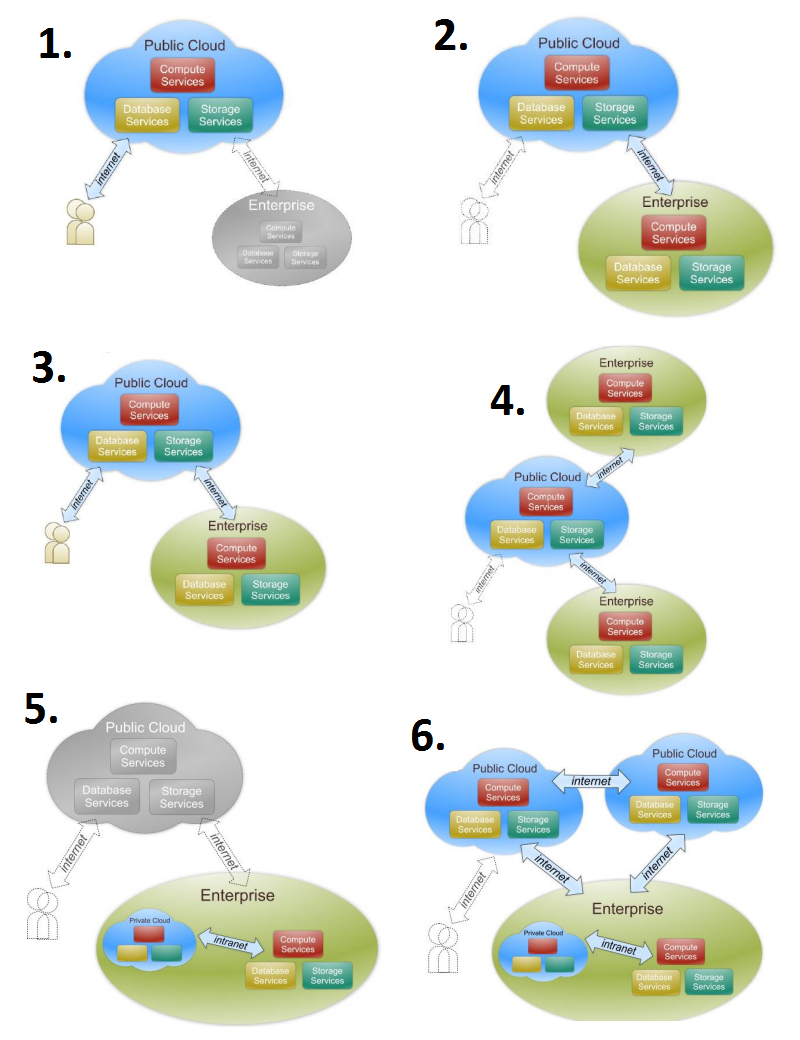
\includegraphics[scale=0.7]{figures/cloud-use-cases.png}
	\caption{Various Use Cases for Clouds and the Different Types of Clouds Available}
	\label{fig:cloud-use-cases}
\end{figure}

\paragraph{\textbf{NOTE: }} A cloud broker could deliver hybrid clouds to users, without the users actually knowing the clouds using underneath . The broker acts as middleman that gets the most optimal resources for the user!

\subsection{Taxonomy}

There are three main types of service layers within a cloud. Any of these 3 service layers can be exposed to the client, and \textbf{lower layers} of the exposed layer are hidden from them.

\subsubsection{Software as a Service}

\textbf{Software as a Service (SaaS)} is an alternative to applications which are traditionally run locally. Users may pay a monthly fee, or for how much resources they use. Examples of Software as a Service would be Salesforce, or Google Docs.

\subsubsection{Platform as a Service}

\textbf{Platform as a Service (PaaS)} is a software stack which facilitates \textbf{deployment of applications}. For example, a web application could be hosted on a cloud provided web server. This removes the responsibility from the client to configure web servers (or other similar software) in a secure manner.

\subsubsection{Infrastructure as a Service}

\textbf{Infrastructure as a Service (IaaS)} is the lowest level in the taxonomy. In IaaS the customer gets access to the virtual machine, and can install their own Operating System and associated software on it. It requires the greatest amount of set up and configuration, but gives the user a greater amount of flexibility. In IaaS the core principals of \textbf{elasticity} still apply, and customers benefit from the networking, physical hardware and other infrastructure resources that the cloud service provider has built up. 

\subsection{Typical Cloud Architecture}

\begin{figure}[h]
	\centering
	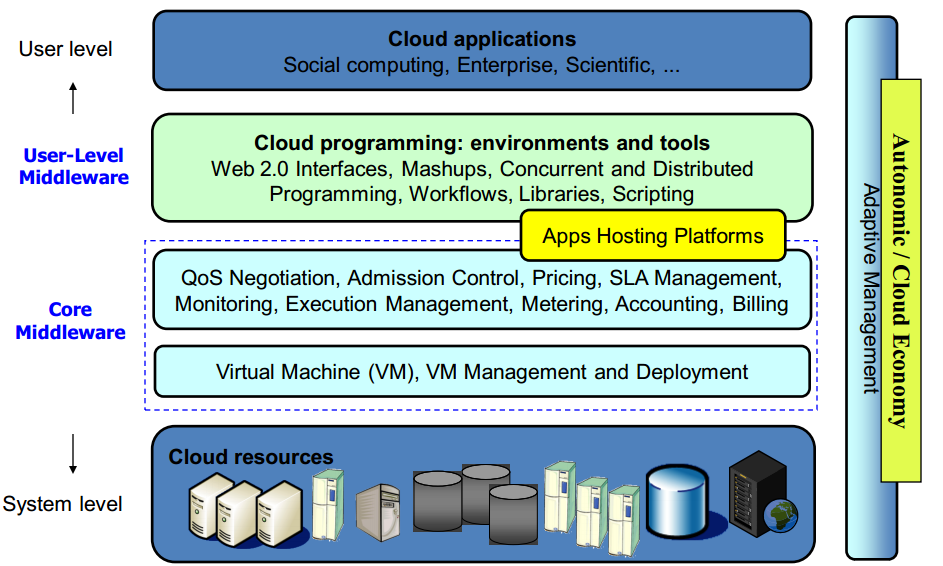
\includegraphics[scale=0.5]{figures/cloud-layered-architecture.png}
	\caption{Layered Cloud Architecture}
	\label{fig:cloud-layered-architecture}
\end{figure}

A typical \textbf{cloud architecture} has four main layers, which from the bottom layer to the top are:
\begin{itemize}
	\item \textbf{System Layer} -- consists of lots of commodity resources, such as computing power, storage and network connections.
	\item \textbf{Core Middleware Layer} -- provides virtualisation (for virtual machines and VM management) and various business functions (Quality of Service, Pricing, metering, SLA Management, Accounting, Billing, etc).
	\item \textbf{Application Development Layer} -- this contains the cloud programming environments and tool, possibly connected to an Application Hosting Platform. This consists of various libraries, workflows and tools which allow applications to be developed for the cloud. 
	\item \textbf{User Application Layer} -- contains the user's developed applications which are currently being deployed and accessed to users
\end{itemize}

\subsection{Virtualisation}

\textbf{Virtualisation} is a key technique in cloud computing, as it allows multiple services to be run on one server in isolation. This includes the isolation of platforms like Windows or Linux, allowing them to \textbf{co-exist simultaneously on the same physical machine}. This \textbf{reduces complexity} and allows for the consolidation of servers, \textbf{reducing cost}. It also allows for quick configuration and administration of servers, as they can be run from a preprepared virtualised image, mounted to a virtual server, rather than having to be created from scratch and installed on physical hardware. Finally, it creates a simplified, sandboxed environment from which \textbf{pay-per-usage business models} can be set up with reasonable simplicity. 

There are 4 types of virtualisation.
\begin{itemize}
    \item Full Virtualisation
    \item Hardware Assisted Virtualisation
    \item Partial Virtualisation
    \item Hybrid Virtualisation
\end{itemize}

A \textbf{virtual machine} is a representation of a real machine using software that provides an operating environment which can run or host guest operating system. A \textbf{guest operating system} is an operating system running in a virtual machine environment that would otherwise run directly on a separate physical system.

The virtualisation layer of the cloud is the\textbf{middleware} between the underlying hardware and virtual machines represented in the system also known as the \textbf{virtual machine monitor (VMM)}.

\subsubsection{Virtual Infrastructure Manager}

A \textbf{Virtual Infrastructure Manager (VIM)} allows resources to be provisioned on behalf of the end user. It stages \textbf{virtual images} (i.e. VMs), creates resources, migrates them and terminates them when necessary. It also \textbf{tracks resource usage} (both physical and virtual) and provides user access control limitations (e.g. you can only use $x$ amount of space or $y$ amount of computing power).

The VIM controls and monitors the physical machines, as well as executing the virtual machines, via a \textbf{secure shell session}. The images necessary to start the virtual machines can be found on a \textbf{network file system}. This level of abstraction allows for physical machines to be added on the fly.

The VIM allows for a \textbf{completely simulated host environment}, meaning you can have multiple virtual hostsm, that apepar as regular hosts to external systems, operating on a single physical host.

\subsubsection{Hypervisors}

The primary technology behind virtualization is a \textbf{hypervisor}. This partitions the (physical) host machine into several simulated hardware environments, which are transparent (can't notice the difference) emulations of a true machine. Examples of hypervisors include VirtualBox, VMWare, Xen, ESX and KVM.

The prime distinction between types of hypervisor is the environment in which they run. Some hypervisors execute "on the metal" (aka, without an operating system), whereas others execute \textbf{within} the operating system as a standard application.

\begin{figure}[h]
	\centering
	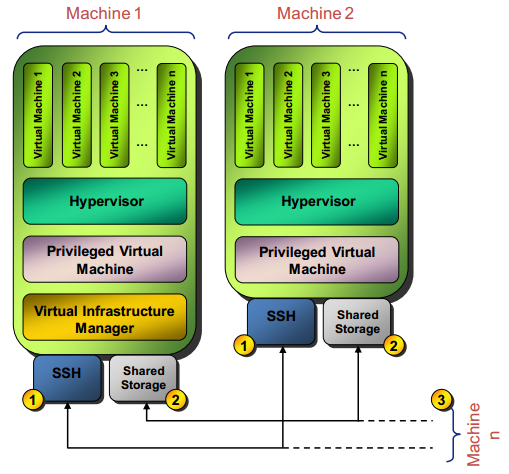
\includegraphics[scale=0.5]{figures/cloud-physical-architecture.png}
	\caption{Physical Architecture of a Cloud}
	\label{fig:cloud-physical-architecture}
\end{figure}

Figure \ref{fig:cloud-physical-architecture} shows the physical architecture of a cloud. The numbered notes on the diagram are as follows:
\begin{enumerate}
	\item \textbf{Virtual Infrastructure Manager} controls/monitors physical machines and executing Virtual Machines via a \textbf{Secure Shell }
	\item Images necessary to start Virtual Machines are shared via a repository on \textbf{Network File System} (e.g. Hadoop/Google File System)
	\item Additional physical machines can be \textbf{added on the fly} as the need arises
\end{enumerate}


\subsection{Standardization}

One key area in which the cloud is not complete is the \textbf{standards} used. Whilst some standards are settled upon (for example, HTTP, REST and Xen) there is still a wide variety of key parts of cloud infrastructure which have not yet received standards.

This may be due in part to the relative youth of cloud computing. Parts of the cloud infrastructure which still need to be standardized include \textbf{virtual image formats}, security and cloud federations. There are efforts to standardize parts of the cloud landscape, including creating open source \textbf{reference} implementations of key parts.
 
\subsubsection{OpenNebula}

OpenNebula is a Virtual Infrastructure Manager which is independent of the hypervisor used. It adopts standard cloud interfaces, and has a flexible, modular architecture. 

It is the VIM used in the School of Computing Cloud Testbed.

\subsubsection{OpenStack}

OpenStack is a Virtual Infrastructure Management tool which aims to become the \textbf{ubiquitous open source cloud computing platform}, by being simple to implement and massively scalable. It hopes to become the "Linux of Cloud Computing Systems". 

It provides a \textbf{management layer} which adds automation and control. It efficiently allocates resources through the system, and empowers both developers and administrators via a wide range of APIs and service portals. It also allows cloud systems to be \textbf{federated} together. In other words, it allows separate clouds from different organisations to combine into a \textbf{cloud federation}.



\section{Big Data}

In modern systems, a great deal of information is being collected and warehoused. The increase in computer usage means that there has been a massive increase in information from sources like social networks, bank transactions, advertising and analytics. Companies such as Google and Facebook are generating terabytes of data every day, and store well into the petabyte regions in total.

Big data doesn't \textit{have} to come from users. It can also come from sensors (like atmospheric sensors for weather ) or large scale simulations.

There is a need to \textbf{manage and analyse}this data to make use of it, requiring automated analysis, visualization or summarisation of vast amounts of data quickly. 

\subsection{Types of Data}

Data can take various forms. \textbf{Relational} data is typically stored in relational database management systems. This means it is stored in tables that contain entities, with relationships spanning across these entities. Relational data can be transactional, and many legacy applications store data in a relational manner. 

Data can also be \textbf{unstructured}, such as text data retrieved from the web or audio/video recordings.

\textbf{Semi-Structured} data has properties from both relational and unstructured data, it will typically have some structure, but be more flexible than the strict relational model. Examples of semi-structured data would be XML or JSON. 

Increasingly, \textbf{graph} data is also becoming relevant. Graph data is typically formed from social networks (a graph representing friendships or connections), links between documents on the web and so on.

Additionally, you also have large quantities of \textbf{streaming data} which is never stored, so you can only scan it once. This is a field known as \textbf{streaming analytics}. 

\subsubsection{Characteristics}

Data can also have various different characteristics. Some data is resting -- there are terabytes of data which needs to be processed, but nothing is being \textbf{added or removed} from it. For example, if a large up front simulation is run, there will be a great deal of data to analyse, but it will not change. In this case the challenge is \textbf{volume}.

Another challenge can be the \textbf{velocity} of data, as it is not always at rest. Some data streams give a system only seconds or milliseconds to process each piece. An example of this would be an application concerned with tweets. If the application takes all the tweets from twitter, it would have to be \textbf{very quick at analysing them} (as it probably only has milliseconds to process each tweet).

Data can also have \textbf{variety}. Some data might be structured, but it may also be merged with unstructured data, or videos. Performing analysis on YouTube may be challenging, because some data is structured (the relationship between a person and their video contributions and comments), some is non-structured text (such as comments and descriptions), some is \textbf{graph based} (connections between users, potentially "likes") and some is multimedia (analysis of the video itself). 

Finally, data can have varying degrees of \textbf{veracity}. It may be incomplete or inconsistent. There could be ambiguities or deception (incorrectly computed values) in the data, or latency could prevent the entire data from being present. Furthermore, the data may be \textbf{out-of-date and not timely}. There may be model approximations, rather than actual data (or alongside actual data). 

\subsection{Requirements}

There are various things which must be done with Big Data.

One typical problem is \textbf{searching} through data, finding relevant information. This typically requires the data to be indexed. It may allow for keyword matching searches (such as hashtags in Twitter) or broader, more powerful pattern matching (such as XML or Regex).

Another use for Big Data is mining it for information, using \textbf{statistical models to determine key facts} from the vast body of information. \textbf{Data mining} may be used, for example, to sell products to customers, or determine which adverts are most suitable to them. These insights would be gained from a great deal of information about the user, such as their website visits, or what products they've purchased in the past.

Finally, data may be aggregated and used for the purpose of statistics. Typically this type of information can be kept in a \textbf{data warehouse}.

\subsection{Challenges}

Most of the requirements have been solved in the past. What makes Big Data unique is the various challenges that it provides:
\begin{itemize}
	\item \textbf{Volume} -- The volume of data in Big Data problems is unprecedented. Existing techniques for using data (querying it, for example) may break down when utilized at this scale. Moreover, the rate of data stored in systems is increasing constantly. Facebook and Google will always have more data coming in, and the volume is therefore ever increasing. Example of a system to deal with storing Big Data is the \textbf{Google File System}.
	\item \textbf{Meaning} -- The data must be described in a meaningful way, which will be helpful both now and in the future. Due to the volume of the data, it cannot simply be changed later on, so metadata must be added to data in order to add semantics, which can be used later on.
	\item \textbf{Intelligent Searching} -- It is important to find content in a suitable period of time. Search engines should be enhanced to use the metadata of information, so that it can search the semantics of content in order to perform search operations in a reasonable time frame.
	\item \textbf{Persistence (What to discard?)} -- Wherever possible, data should be discarded. This has the net effect of making the size of the data smaller, and therefore easier to operate upon. Some data may not be relevant to an application, or might not be required again. Some data could be created whenever it is needed, rather than being stored. The cost of processing (to recreate the data) may be outweighed by the impact of storing more data.
	\item \textbf{Governance} -- The management of the information and knowledge contained within storage. Issues such as the quality of the incoming data is important, as the quality of what you put in affects the quality of the insights you derive. This makes governing \textbf{quality control} important.
\end{itemize}

\subsection{MapReduce}

One model for running massively scalable, distributed \textbf{computations} across a large amount of data is called \textbf{MapReduce}. The principal of MapReduce is to:
\begin{enumerate}
	\item break a task down into lots of chunks
	\item execute a function across all of them in parallel (\textbf{map})
	\item reduce the resulting values down into 1 value (\textbf{reduce}).
\end{enumerate}
An example of a (very simple) map reduce job would be to take a sequence of numbers, double them (map a double function across the sequence) and then sum them (reducing them into one value).

Figure \ref{fig:mapreduce} shows a single master process dividing the work up and allocating it to a number of worker/slave processes. Once they've finished processing the given data, they sent the results back to the master process who \textbf{aggregates the results into the final insight/value}. This makes MapReduce is an architectural pattern designed to solve concurrent problems using a master-slave approach.

\begin{figure}
	\centering
	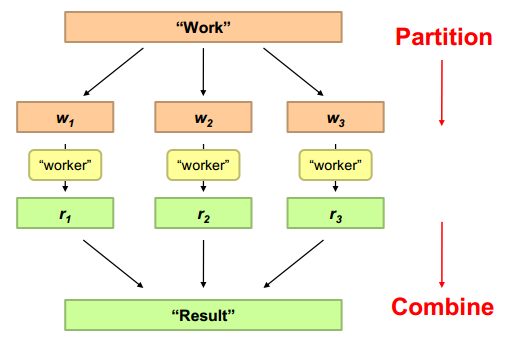
\includegraphics[scale=0.6]{figures/mapreduce.png}
	\caption{Typical Mapreduce Process -- Partition the Work, Solve Sub-Problems Individuall and Combine into a Whole Solution}
	\label{fig:mapreduce}
\end{figure}

MapReduce is well suited to large data processing problems, like those typically found in Big Data, because \textbf{parallelising the processing} to speed up the computation (and not overload an individual machine with that much memory) makes deriving insights \textbf{feasible}. It uses \textbf{divide and conquer} to enable the scalability Big Data demands.

\subsubsection{Hadoop}

\textbf{Hadoop} is a data processing framework built on the idea of MapReduce. It was initially created by Yahoo, and has now been open sourced. Hadoop clusters can be provided \textbf{on-demand in the cloud}, which lowers the barrier to entry to solving Big Data problems. This allow companies to easily derive insights into and scale their usage depending on the amount of data they have (which could grow/shrink unexpectedly due to unpredictable markets).

\subsubsection{Concurrency}

Concurrency is used in order to keep the system efficient. The primary advantage of MapReduce is that it can be parallelised fairly trivially. This is achieved by running the map command across many machines, using a \textbf{function} that does not require data from any other process. However, some problems can still have parallelisation challenges (such as having to communicate partial solutions).

The reduce step of the process is also more difficult to parallelise, as it is implied that all map stages must be completed. Sometimes, the reduce step can be divided into multiple reduce steps, which divide and conquer the process. For example, in the simple double and sum problem, results can be reduced together (summed) as soon as they have been doubled. These \textbf{partial reductions/aggregations} allow calculation to happen asynchronously (without blocking waiting for maps to finish) and in parallel, increasing performance.

\subsubsection{High Level Abstraction}

All of this provides a high level abstraction for the programmer, who no longer has to worry about the \textbf{standard issues with concurrency} (such as deadlocks, race conditions, debugging concurrent problems, etc) and can merely worry about specifying what computation needs to happen (rather than how it is distributed and ran concurrently). 

The programmer provides 2 functions which define the computation which must be performed:
\begin{equation}
\begin{aligned}[b]
	\text{map}(k, v) \rightarrow <k', v'>* \\
	\text{reduce}(k', v') \rightarrow <k', v'>*
\end{aligned}
\end{equation}
The execution framework (such as Hadoop) handles the rest. 

Usually the programmer will also specify a \textbf{method to partition the data}, in order to control how it is sent to nodes. They will also provide a \textbf{combine function}, which acts as a mini-reduce (in memory of the map node) in order to reduce on network traffic:
\begin{equation}
\begin{aligned}[b]
	\text{partition}(k', \text{number of partitions}) \rightarrow \text{partition for }k \\
	combine(k', v') \rightarrow <k', v'>*
\end{aligned}
\end{equation}

\begin{figure}[h]
	\centering
	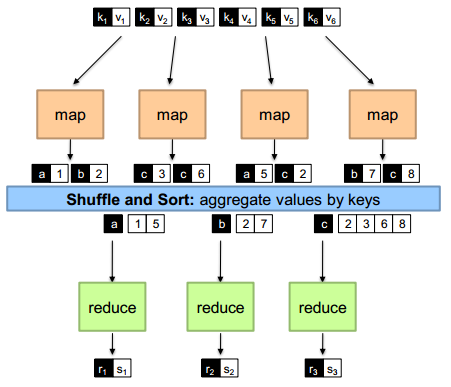
\includegraphics[scale=0.6]{figures/mapreduce-detailed.png}
	\caption{Example of Mapreduce with Specific Array of Data}
	\label{fig:mapreduce-detailed}
\end{figure}

The MapReduce \textbf{runtime} (such as Hadoop) will usually be responsible for scheduling workers to handle map jobs (and partial reduces), moving the data to the appropriate processes (distributed) and any synchronization that needs to occur. It will also handle faults, such as if a worker fails. This makes it easier for application developers to create systems that process Big Data.

\paragraph{\textbf{NOTE: }} It is common to have the Mapreduce work in a tree-like fashion. A master process (root) partitions work to given to other machines (children), who then partition the work \textit{again} and distribute it to more machines. The aggregated/combined partial solutions are then propagated up the tree until the master receives the fully constructed solution.

\subsubsection{Distributed File System}

A \textbf{Distributed File System} is a way of solving the problem of \textbf{moving} data around the MapReduce cluster. In Big Data problems, it would take an unfeasibly long time to move all of the data to the appropriate workers. Instead of doing this, data is stored in the \textbf{nodes which will process said data} to begin with. When a computation is taking place, nodes merely perform the action on data that they \textbf{already have stored}. This is known as:
\begin{quote}
	\textit{"moving the processes to the data"}
\end{quote} 

For Hadoop, the underlying distributed file system is HDFS (Hadoop Distributed File System). 

Google use a proprietary technology called GFS (Google File System), which relies on large amounts of commodity hardware (instead of blades, or other server equipment) which are designed to be fail-able. Each machine stores in the order of gigabytes, and performs MapReduce jobs on its contents using Google's proprietary MapReduce solution.

\end{document}